%%%%%%%%%%%%%%%%%%%%%%%%%%%%%%%%%%%%%%%%%%%%%%%%%%%%%%%%%%%%%%%%%%%%%%%%%%%%%%%%%%%%%%%%%%%%%%%%%%%%
% 
% PRL presentation template
% based on https://github.com/FAU-AMMN/fau-beamer by Tim Roith
% Adaptation done by:
% Linda Schneider
% Dalia Rodriguez-Salas
% Noah Maul
%
% This program can be redistributed and/or modified under the terms
% of the GNU Public License, version 2.
%
%%%%%%%%%%%%%%%%%%%%%%%%%%%%%%%%%%%%%%%%%%%%%%%%%%%%%%%%%%%%%%%%%%%%%%%%%%%%%%%%%%%%%%%%%%%%%%%%%%%%

%\documentclass[handout, notes, t]{beamer}
%\documentclass[notes=only, t]{beamer}
\documentclass[handout, t]{beamer}
%\documentclass[t]{beamer}

%\setbeameroption{show only notes}

\usepackage[utf8]{inputenc}
\usepackage[T1]{fontenc}

%%%%%%%%%%%%%%%%%%%%%%%%%%%%%%%%%%%%%%%%%%%%%%%%%%%%%%%%%%%%%%%%%%%%%%%%%%%%%%%%%%%%%%%%%%%%%%%%%%%%
%% VON MIR
%%%%%%%%%%%%%%%%%%%%%%%%%%%%%%%%%%%%%%%%%%%%%%%%%%%%%%%%%%%%%%%%%%%%%%%%%%%%%%%%%%%%%%%%%%%%%%%%%%%%
\usepackage{enumitem}
\usepackage{booktabs}
\usepackage{float}
\usepackage{nameref}
\newcommand{\Emph}[1]{\textbf{#1}}
\newcommand{\mynote}[1]{\note{\huge{#1}}}
\newcommand{\spacy}{\texttt{spacy}}
\newcommand{\onehot}[1]{$ 1 $-hot-encoded vector{#1}}

\newcommand{\os}[1]{\onslide<+->{#1}}
\newcommand{\Os}[2]{\onslide<#1->{#2}}

\newcommand*{\figref}[1]{\figurename~#1}

%\setbeamercovered{transparent=0}

%\usepackage{xspace}
%\newcommand{\ie}{i.\,e.,\xspace}
%\newcommand{\eg}{e.\,g.,\xspace}

%%%%%%%%%%%%%%%%%%%%%%%%%%%%%%%%%%%%%%%%%%%%%%%%%%%%%%%%%%%%%%%%%%%%%%%%%%%%%%%%%%%%%%%%%%%%%%%%%%%%
%% STYLE
%%%%%%%%%%%%%%%%%%%%%%%%%%%%%%%%%%%%%%%%%%%%%%%%%%%%%%%%%%%%%%%%%%%%%%%%%%%%%%%%%%%%%%%%%%%%%%%%%%%%

% the possible options for the 'i2beamer' package are:
% - 'english' (if the slides are in english) 
% - 'wide'    (if the slides should use a 16:9 aspect ratio)
% - 'logo'    (if the logo of the Programming Systems Group should be included)
% - 'plain'   (if the background image of the title page should be omitted)
% - Faculty shorts: nat, phil, med, tf, rw, wiso, jura (no faculty short results in FAU)

\RequirePackage[wide,logo,tf,english]{sty/beamer}

% VON MIR
% Nachfolgende Stichpunkte schimmern nicht in grau durch
% Muss NACH \RequirePackage{.../beamer} stehen
\setbeamercovered{transparent=0}

%%%%%%%%%%%%%%%%%%%%%%%%%%%%%%%%%%%%%%%%%%%%%%%%%%%%%%%%%%%%%%%%%%%%%%%%%%%%%%%%%%%%%%%%%%%%%%%%%%%%
%% Bibliography
%%%%%%%%%%%%%%%%%%%%%%%%%%%%%%%%%%%%%%%%%%%%%%%%%%%%%%%%%%%%%%%%%%%%%%%%%%%%%%%%%%%%%%%%%%%%%%%%%%%%
\defbibheading{bibliography}{}
\addbibresource[label=primary]{references.bib}
\nocite{*}

%%%%%%%%%%%%%%%%%%%%%%%%%%%%%%%%%%%%%%%%%%%%%%%%%%%%%%%%%%%%%%%%%%%%%%%%%%%%%%%%%%%%%%%%%%%%%%%%%%%%
%% INFO
%%%%%%%%%%%%%%%%%%%%%%%%%%%%%%%%%%%%%%%%%%%%%%%%%%%%%%%%%%%%%%%%%%%%%%%%%%%%%%%%%%%%%%%%%%%%%%%%%%%%

\title{\parbox{\textwidth}{The hippocampus and language: Word to word prediction in terms of the successor representation}}
%\subtitle{Optional subtitle of document}

\author{Philipp Rost}
\institute[Department Informatik]{Friedrich-Alexander-Universität Erlangen-Nürnberg\\ Department Informatik}
%\institute{Friedrich-Alexander-Universität Erlangen-Nürnberg}

\date{\today}

%%%%%%%%%%%%%%%%%%%%%%%%%%%%%%%%%%%%%%%%%%%%%%%%%%%%%%%%%%%%%%%%%%%%%%%%%%%%%%%%%%%%%%%%%%%%%%%%%%%%
%% DOCUMENT
%%%%%%%%%%%%%%%%%%%%%%%%%%%%%%%%%%%%%%%%%%%%%%%%%%%%%%%%%%%%%%%%%%%%%%%%%%%%%%%%%%%%%%%%%%%%%%%%%%%%

\begin{document}

% === TITEL FOLIE ===================================

\begin{frame}[plain,c]
  \titlepage
\end{frame}

% === AGENDA ===================================

\begin{frame}
    \frametitle{Agenda}
    \tableofcontents
% --- NOTIZEN -----------------------------------
\mynote{
    \begin{itemize}
        \item[ü] The agenda consists of five sections: Introduction, the theoretical background, presenting the framework I have developed, my results and a conclusion 
    \end{itemize}
}
\end{frame}

% === INTRODUCTION ===================================

\section{Introduction}
\begin{frame}{Introduction}
    \begin{itemize}
    	\item<+-> Understanding the human brain is a challenge as old as science itself
    	\item<+-> Currently available technology as a metaphor (from abacus to computer)
    	\item<+-> Projects exist researching the brain as a whole but also for distinct parts, e.g. the hippocampus
    	\item<+-> Goal: Expanding the application of the Successor Representation (SR) to language
    	\begin{itemize}
    		\item<5-> supposedly used by the hippocampus to predict following states/positions
    	\end{itemize}
    	\item<6-> To reach it, a neural network is trained with samples extracted from two books
    \end{itemize}
% --------------------------------------
\mynote{
\begin{itemize}
    \item[ü] I will start with a short overview
	\item Understanding the human brain is a challenge as old as science itself
	\item Currently available technology serves as a metaphor (from abacus to computer)
    \item There exists projects researching the brain as a whole but also for distinct parts, e.g. the hippocampus
	\item The goal of my thesis is the expansion of the Successor Representation. STICHPUNKT EINBLENDEN Via the SR we can kinda predict future states/positions in an environment, for example our location in a city. The technique was applied beforehand successfully to a spatial environment and shall now be extended to an abstract scenario like language. To put in bluntly, is it possible to achieve proper (long term) word to word predictions by this technique?
	\item To reach it, a neural network is trained with samples extracted from two books
\end{itemize}
}
\end{frame}

% === CHAPTER ===================================

\chapter{Theoretical Background}

% ======================================

\section{Hippocampus} \label{sec: Hippocampus}
The hippocampus is located in the brain and part of an old area called the archicortex. It is named after the greek word for seahorse, because it has the shape of one (\figref{\ref{wrapfig: Hippocampus and seahorse}}). This brain area can be divided into three parts: the dentate gyrus, the cornu ammonis and the subiculum~\cite{ORFrHa20CCN, GarzorzStark18BN}.

\begin{wrapfigure}{r}{0.35\textwidth}
	\centering
		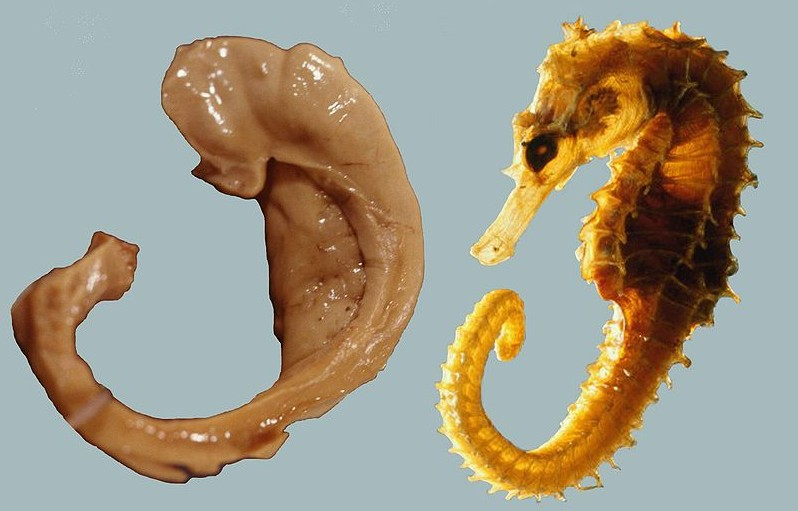
\includegraphics[width=0.35\textwidth]{Hippocampus_and_seahorse.jpg}
	\caption{Hippocampus and seahorse~\cite{Seress10H}} % TODO Besser formatieren oder entfernen
	\label{wrapfig: Hippocampus and seahorse}
\end{wrapfigure}
The hippocampus plays a fundamental role in forming new memories (not preserving them, which is done across the brain) and is highly capable of learning new information fast. Regarding its functions, one was already mentioned: It is the key area when it comes to establishing new memories. Patients with a damaged hippocampus, therefore lacking this ability, will lose spatial and temporal orientation. Moreover epilepsy, schizophrenia and Alzheimer's disease are connected to this dysfunctional organ~\cite{Trepel17N}.
The hippocampus is also important in emotional contexts because it is an integral unit of the limbic system~\cite{GarzorzStark18BN}. Another task, and for this thesis the most important one, is navigation/orientation, not just in spatial surroundings, but also in an abstract context, called \cognitiveroom{}. Some examples for abstract contexts are: Danger of animals based on their appearance and speed of vehicles based on their weight and engine (\secreff{sec: predictive map theory}). To achieve this skill, two types of cells in the hippocampus are active: place cells and grid cells.
The first one encodes states/positions (one for each cell) and the latter resembles a coordinate system.
\paragraph{Place cells} \label{par: Place cell}
Place cells are irregular distributed across the cognitive room. Their firing is tied to the location of the state, whereby the term location has not always its classic spatial meaning if we navigate in an abstract setting (as mentioned above). The place cell is active in case we encounter the associate state. As seen in \figref{\ref{fig: Rat in maze}}, different place cells (each is color coded) fire at different positions in the parkour \eg turquoise is undoubtedly related to the first arch, meaning its activity spikes while the rat passes by. The remark of the thesis lies on place cells.
\begin{figure}
	\centering
		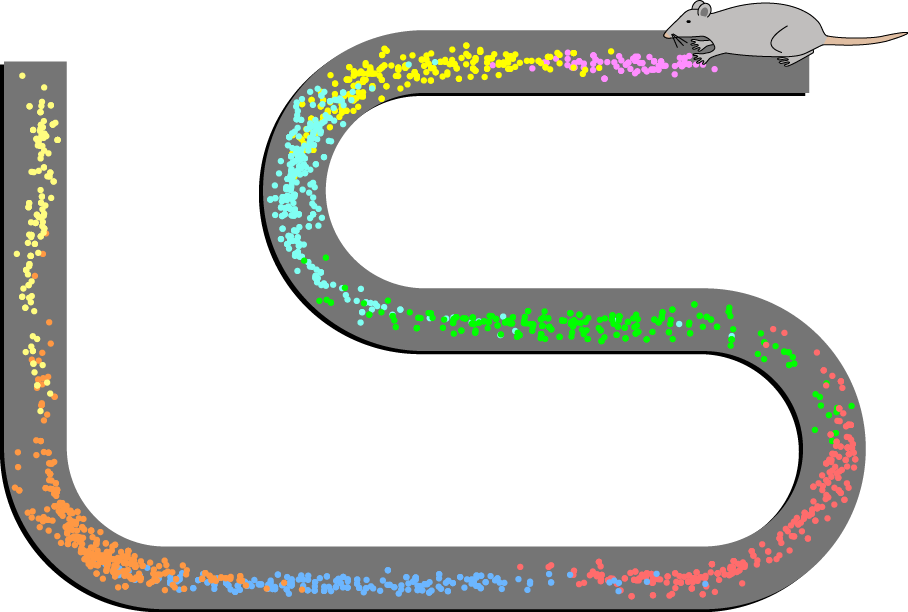
\includegraphics{Ortszelle_Beispiel.png}
	\caption{Activity pattern of color encoded place cell across a maze. Each place cell is exactly related to one distinct position of the corresponding environment \eg turquoise to the first arch. Its activity spikes if the rat walks along the arch~\cite{Stuartlayton13}.}
	\label{fig: Rat in maze}
\end{figure}
%This means in a spatial scenario, where we walk around in a square \TODO[fancyline]{Bild in GeoGebra erstellen mit Quadrat, Brunnen, Baum..., daneben Aktvierungsmuster der Ortszellen} (i.e. with a fountain), it fires irregularly and always then if we are at the position the place cell encodes. In case it resembles the fountain it will fire if we are close to it. \\
\paragraph{Grid cells}
This type of cell can be found in the entorhinal region and satisfies a more general purpose. They are regularly distributed and form a triangular lattice (\figref{\ref{fig: Grid cells}}). It provides raw spatial information in terms of a metric or distance measure the hippocampus integrates with the place cells~\cite{ORFrHa20CCN, BellmundEtAl18NC}.
\begin{figure}
	\centering
		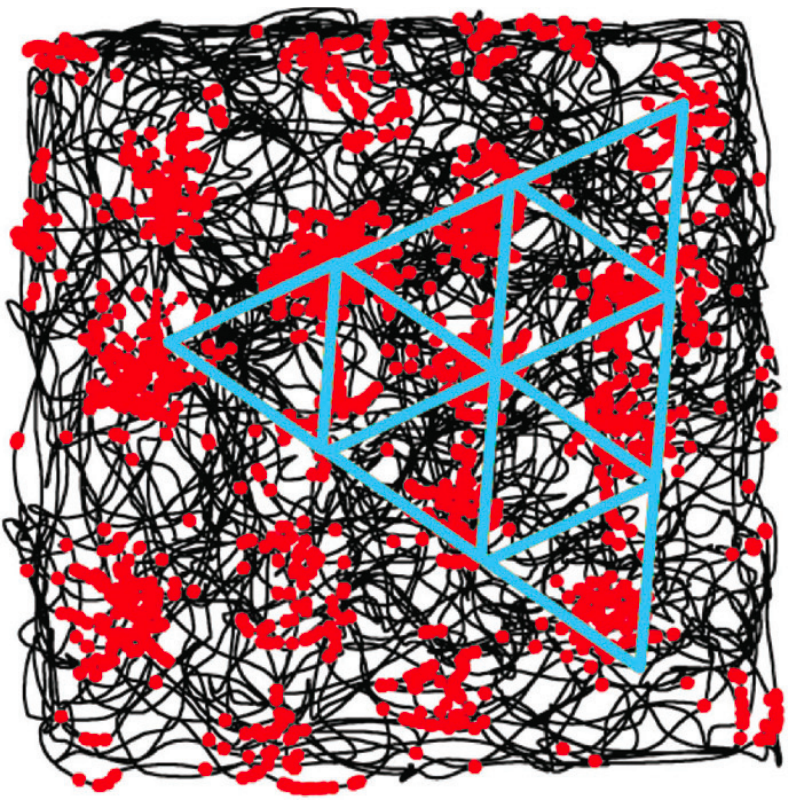
\includegraphics[scale=0.25]{Gitterzelle_Beispiel.png}
	\caption{Sketched path of a rat moving in a square, while tracking firing grid cells. As their name suggests, they form a regular lattice over the space. Hence, they act as coordinate system. The information provided by grid cells is combined with that of the place cells to generate a full picture of the surroundings~\cite{Moser15PGM}.}
	\label{fig: Grid cells}
\end{figure}


% ======================================

\section{Predictive map theory} \label{sec: predictive map theory}
To explain the principle of the predictive map theory introduced in~\cite{StBoGe17HPM}, it is necessary to illustrate the concept of a \cognitiveroom{}, mentioned before in \secreff{sec: Hippocampus}. An example is of course a naive navigational task as presented by \etal{Stachenfeld} and similar to the setting of \figref{\ref{fig: Rat in maze}}. The authors even demonstrated that just a topological environment is sufficient to craft a \cognitiveroom{} and apply the predictive map theory.

The concept becomes far more interesting when talking about cognitive rooms founded on experience \ie the speed of vehicles based on weight and engine specifications. This category of a \cognitiveroom{} also fits the topic of the thesis much better, since it aims to model language not a spatial environment. An illustrating example can be found in \figref{\ref{fig: vehicles cognitive room}}. For instance, a ``sports car'' might be rather lightweight but has plenty of horse power.
\begin{figure}
	\centering
		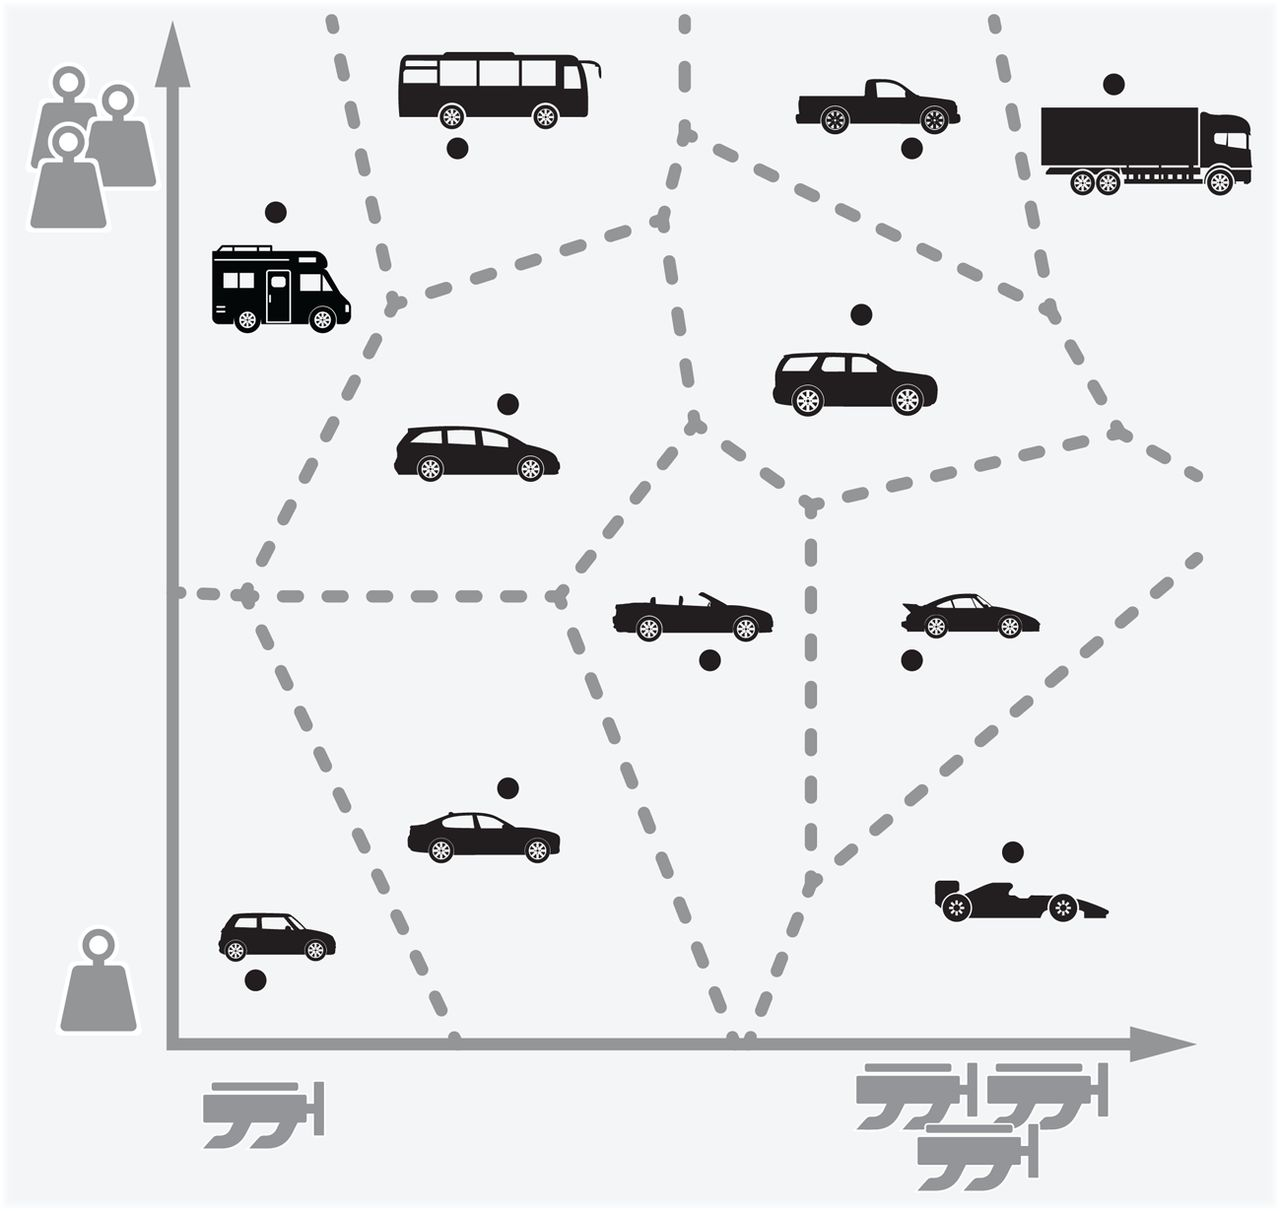
\includegraphics[width=0.4\textwidth]{Fahrzeuge_Cognitive_Room.jpeg}
	\caption{Exemplary \cognitiveroom{} of vehicles according to their weight and engine power. An unknown car can be placed easily in the environment given the two parameters because there are already established place cells acting as abstract waypoints (the depicted cars) to support the orientation \ie finding its place on the map. By doing so, it is immediately possible to derive information about the appearance of the automobile~\cite{BellmundEtAl18NC}.}
	\label{fig: vehicles cognitive room}
\end{figure}
By using these two characteristics, the \cognitiveroom{} has the shape of a $ 2d $-plane. For instance, while reading about an alien car, it is immediately possible to compare it with different well-known vehicles and draw conclusions about its shape since the \cognitiveroom{} has enough information to position the car within it. All these decisions of placing new objects in an appropriate context is done by place and grid cells (\secreff{sec: Hippocampus}). Expanding the example by the firing of cells results in the full illustration given in \figref{\ref{fig: vehicles with place and grid cells}}.
\begin{figure}
	\centering
		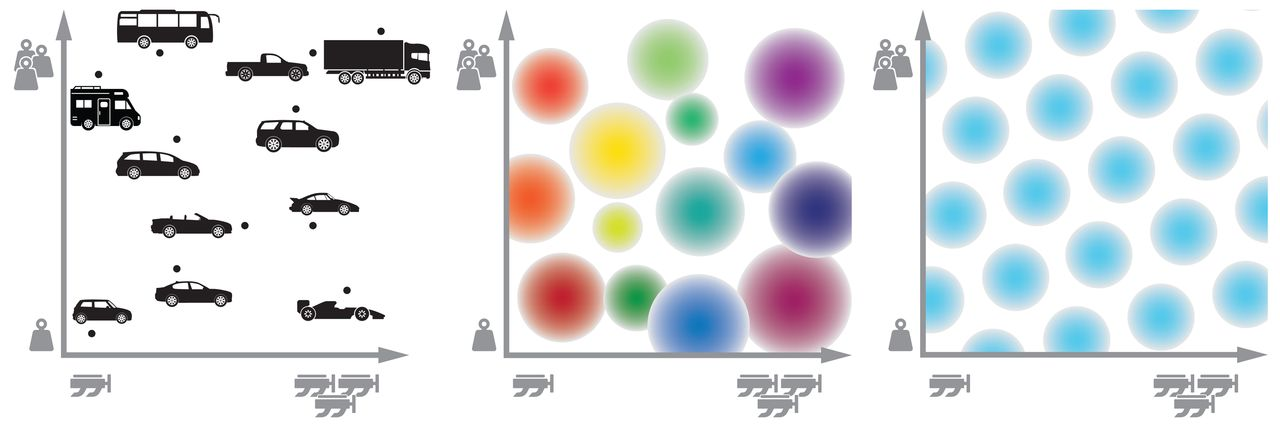
\includegraphics[width=1.\textwidth]{Fahrzeuge_Ortszelle_Gitterzelle.jpeg}
	\caption{Left: \cognitiveroom{} of vehicles according to weight and horse power. Middle: Firing pattern of place cells crafting the \cognitiveroom{} \ie the boundaries in \figref{\ref{fig: vehicles cognitive room}}. Right: Corresponding lattice of grid cells.~\cite{BellmundEtAl18NC}}
	\label{fig: vehicles with place and grid cells}
\end{figure}

%
% Paul bezieht die „Prdictive Map theory“ lediglich „auf die Autos und Tiere“
%

%In case of encountering a unknown species the predictive map becomes active in terms of firing place cells encoding animals sharing the same features and thus evaluating the potential danger. In these terms a place cell doesn't encode the current state but a future state because the new living being will be cataloged next to the known ones. So, the cognitive room exhibits a predictive property.
%
%We can, for instance, apply it to the scenario of the rat passing a maze as seen in Fig. \ref{fig: Rat in maze}. In par. \nameref{par: Place cell} was mentioned that a place cell resembles the current position. By the new perspective follows that the cell fires beforehand~\eg again in terms of the turquoise cell: This cell is now contemplated active if the rat is within the are preceding the arch and aims to enter it.
%
%Furthermore, the authors argue that


% ======================================

\section{Successor Representation} \label{sec: SR}
According to \etal{Stachenfeld}, our behavior in an open spatial environment, or in general in a \cognitiveroom{} \eg a city, follows the predictive map theory introduced in \secreff{sec: predictive map theory}. An active place cell encodes the next/successor state entered by the agent.

To model this or the general setting of predicting future states, the \gls{sr} was developed by a \gls{rl} approach. Furthermore, the \gls{sr} and the predictive map theory go hand in hand. The latter is an application regarding the former: The authors support the proposition that hippocampal mechanics, explained by the predictive map theory, can be described via the \gls{sr}.

% ======================================

\subsection{Mathematical Foundation}
The basis lies largely in \gls{rl}, in formula:
\begin{equation}\label{eq: rl}
	V(s) := E \left[
				\sum_{t=0}^{\infty}
					\gamma^t R(s_t) | s_0 = s
			\right]
\end{equation}
with $ V $ resembling a value function, expressed via the reward function $ R $, which operates on state $ s_t $, encoded by the sum over $ t $, starting in $ s $. $ \gamma \in [0,1] $ serves as a discount factor to control the influence of states reached in distant future. High values permit distal states to play a larger role, whereas smaller values de facto limit the result to neighboring positions\footnote{Short mathematical explanation: $ p^t \xrightarrow[]{t \to \infty} 0 $ for $ p \in [0,1) $, the greater $ p $ the slower happens the approach of the limit. For $ p = 1 $ the sequence is constant. In our case every state is taken into account equally.}. By the reward function is obtained how beneficial the currently visited state $ s_t $ is. % The expected value is taken because there are \wlog plenty of paths starting in $ s $.
After the calculation of $ V $, the function can be decomposed into a more intuitive representation, consisting of a state matrix $ M $, called the \srmat{}, and the known reward function $ R $:
\begin{equation}\label{eq: v with sr-matrix}
	V(s) = \sum_{s'}
				M(s, s') \cdot R(s')
	\text{.}
\end{equation}
The first argument of $ M $ specifies the row, the latter the column. Each cell contains the discounted expected number of times the agent visits state $ s' $ starting from $ s $. Additionally, \etal{Stachenfeld} mention that the \srmat{} can be derived from a transition probability matrix $ T $ for the positions $ s $~\cite{StBoGe17HPM}. Having $ T $, it follows
\begin{equation}\label{eq: sr or m via T}
	M = \sum_{t = 0}^{\infty}
			\gamma^t T^t
	\text{,}
\end{equation}
which is a geometric series and converges for $ \gamma < 1 $ towards
\begin{equation}\label{eq: geo series}
	(I_n - \gamma T)^{-1}
	\text{,}
\end{equation}
where $ I_n $ is the corresponding identity matrix.

Although defining all formulae by infinite sums, it is seamlessly possible to calculate the \srmat{} in \equref{\eqref{eq: sr or m via T}} up to a finite index or starting at an arbitrary $ t $ \ie $ t=1 $. Doing so makes sense in a language environment. The identity matrix would imply that a word can follow itself, which is extremely rare\footnote{Although sentences like ``Ich hoffe, dass das das Richtige ist.'' do occure in german.}. Therefore, the first summand will always be $ \gamma T $, where $ T $ is calculated by a Neural Network (\secreff{ch: framework}). If the indices in \equref{\eqref{eq: sr or m via T}} are altered, the limit of the geometric series no longer applies directly and has to be adjusted by subtracting the first summands from \equref{\eqref{eq: geo series}}. The \gls{sr} and thus the depicted formulas, especially the \srmat{} and the transition probability matrix, are policy dependent. This is reflected by the training data.

By definition, matrix $ M $ reveals all successor states with their particular probability because the summation combines the following positions, which are calculated by exponentiation, into one matrix. By examining a row (\figref{\ref{fig: sr-spalte}}) \eg row $ k $, it is possible to follow all paths starting from state $ k $.

One advantage of the \gls{sr}, \ie describing the model by the \srmat{} $ M $, is its high flexibility regarding the evaluation of different reward functions given by \equref{\eqref{eq: v with sr-matrix}}. The value of a state $ s $ can be calculated in an instant with a different reward function while no relearning is necessary.

\paragraph{\gls{sr} and grid cells}
Although not further discussed in the thesis but an interesting claim of \etal{Stachenfeld} is that the eigenvalue decomposition of the \srmat{} reveals the grid cell structure. They provide supplementary information depicting many examples~\cite{StBoGe17HPM}.

% ======================================

\subsection{Example for the Successor Representation}
This subsection is dedicated to fill the concept of the \gls{sr} and the \srmat{} $ M $ with some intuition. \etal{Stachenfeld} simulated a linear spatial environment built by six states with a simple policy merely consisting of two actions the agent can apply: Going one step to the right or pausing.
%
\paragraph{Rows}
In this scenario, a plot of single rows of $ M $ is shown in \figref{\ref{fig: sr-zeile}}.
\begin{figure}
	\centering
		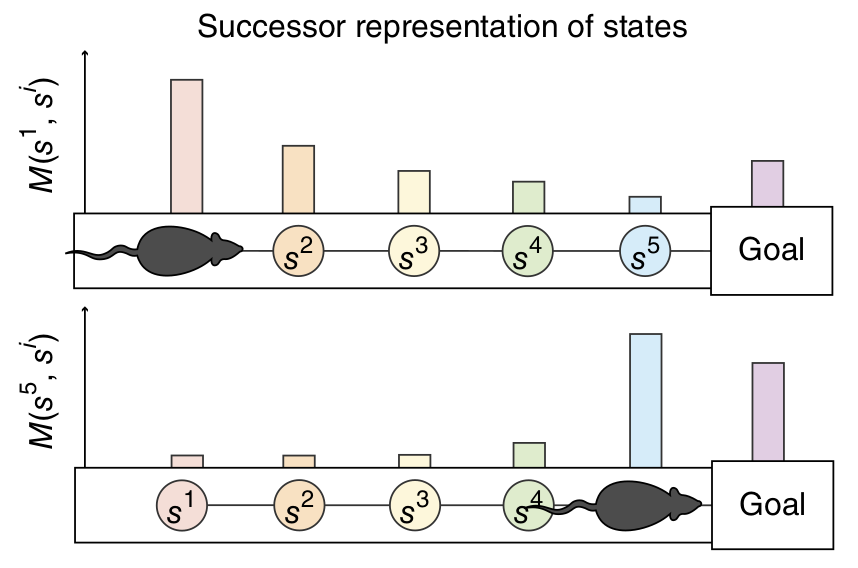
\includegraphics[width=0.7\linewidth]{Beispiel_SR_Zeile.png}
	\caption{Schematic plot of the rows of state $ s^1 $ and $ s^5 $ respectively. By interpreting the ordinate values as probabilities for transitioning instead of a probability for the current state, it is possible to make assumptions on the future path the agent may take. Hence, matrix $ M $ describes all possible paths. In both cases the policy prefers pausing over changing the state.}
	\label{fig: sr-zeile}
\end{figure}
From the upper half of \figref{\ref{fig: sr-zeile}}, examining the row of $ s^1 $, it is possible to deduce that the agent will most likely remain at its current position, with the values for distal locations disappearing. A different point of view results for the part of $ M(s^5, s^i) $. It is obvious that going backwards is nothing to reckon with since the numbers for transitioning distribute over $ s^5 $ and \texttt{goal} by slightly favoring the former. This behavior was expected by the policy.
%
\paragraph{Columns}
It is also worth analyzing the columns of $ M $, called \emph{place fields} by \etal{Stachenfeld} (\figref{\ref{fig: sr-spalte}}). Having the policy in mind, it is no surprise that the values $ M(s^i, s^5) $ ascend in parallel to the index $ i $. The probability for entering $ s^5 $ grows by approaching it. In addition the plot shows how $ s^5 $ is probably reached best, simply by passing via $ s^3 $ and $ s^4 $. This might seem obvious, but in a more complex \cognitiveroom{} the graph won't look as ordinary and therefore will contain plenty of distributed information. %A spike on $ s^1 $ would counteract it because it means stepping from $ s^1 $ to $ s^5 $ directly (as seen in Fig. \ref{fig: sr-zeile} this is not the case).
\begin{figure}
	\centering
		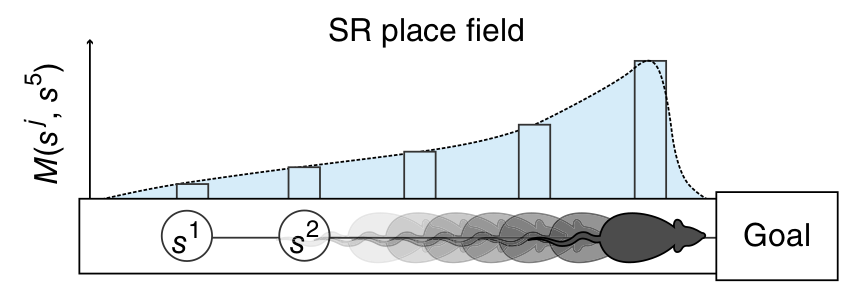
\includegraphics[width=0.7\textwidth]{Beispiel_SR_Spalte.png}
	\caption{Schematic plot of the $ s^5 $-column depicting how $ s^5 $ is reached by ascending probabilities. It is possible to recapitulate the policy consisting of pausing or taking one step to the right. Entering $ s^5 $ is most likely from $ s^4 $ and $ s^5 $ (due to resting). }
	\label{fig: sr-spalte}
\end{figure}


% ======================================

\section{Multidimensional Scaling}
The goal of \gls{mds} is to calculate a $ m $-dimensional mapping, $ m < n $, of a given point cloud in $ \mathbb{R}^n $ that preserves the original distances as good as possible~\cite{HaTiFr17ESL}. The result of the calculation is unique modulo rotation and scaling. Therefore, it is based on a metric and not exact coordinates. \gls{mds} is used to analyze similarities between the rows of the \srmat{} by determining clusters in the graph.\\
%
The algorithm is simple and only uses basic linear algebra. \gls{mds} works with a distance matrix $ D $, where each entry is equal to $ d_{ij}^2 $, the squared distance between two points $ x_i, \ x_j \in \mathbb{R}^n $, whose coordinates are (in principle) unknown. By double centering $ D $ it is possible to calculate the matrix product $ X^\top X $, where $ X $ bears the coordinates in the desired dimension~\cite{Riess20PA}. Double centering means multiplying by a matrix $ C := I_n - \frac{1}{n}J_n$, where $ J_n $ is a $ n \times n $-matrix of ones:
\begin{equation}
	\underbrace{-\frac{1}{2} CDC}_{B :=} = X^\top X
	\text{,}
\end{equation}
The centering matrix $ C $ has, after a multiplication with a column vector, the same effect of subtracting the mean of all components from the vector itself. \\
In the next step, the $ m $ largest eigenvalues of $ B $ are calculated along with their corresponding eigenvectors. Finally, the $ m $-dimensional coordinates are determined:
\begin{equation}
	X_m = E_m V_m^{1/2}
	\text,
\end{equation}
where $ E_m $ contains the $ m $ eigenvectors and $ V_m $ is a $ m $-dimensional diagonal matrix with the associated eigenvalues.


% ======================================

\section{Metric for quantifying the results} \label{sec: metric}
Throughout the presentation of the results in \chapreff{ch: results} numerous matrices and \gls{mds} plots are used. Sometimes, they give a clarifying visual response, but not in all cases. When comparing different approaches, images lack the needed objectivity and plausible criteria to rate the outcomes. To tackle this issue, a metric was developed to have the possibility to draw objective conclusions.

Since Neural Networks on languages are trained, a measure on the grade of the closeness to the real counterpart is necessary, which is referred by ``ground truth (distribution)'' in the following. The mathematical objects are in both cases squared matrices of dimension $ n \in \mathbb{N} $ built by transposed probability vectors. Nevertheless, the presented mapping is made for $ n \times m $-matrices. Depending on the model type, the ground truth vectors are \onehot{s} or share different fractions across all entries (\secreff{sec: w2w models}).

Hence, the starting positions for the metric are probability vectors. The obvious way to quantify the results is by taking the euclidean norm $ d $ of the difference of the ground truth and the prediction. Consequentially, $ d $ takes values between $ 0 $ and $ \sqrt{2 \cdot n} $ because the maximal difference for each row is $ \sqrt{2} $ and there are $ n $ in total. $ \sqrt{2} $ is derived by the following nonlinear program
\begin{align}
	\mathrm{max} 	& \quad \Vert \vec{x} - \vec{y}\Vert_2 = \sqrt{\sum_{i=1}^{n} (x_i - y_i)^2} \nonumber\\
	\mathrm{s.t.} 	& \quad \sum_{i=1}^{n} x_i = 1, \ \sum_{i=1}^{n} y_i = 1\\
					& \quad x_i, y_i \in [0,1] \nonumber
	\text{,}
\end{align}
which is solved by \onehot{s} for $ \vec{x} $ and $ \vec{y} $ where $ x_i = 1 \neq y_i$ for a $ i \in \{1, \ ..., \ n\} $. Or to put it bluntly, the difference takes its highest values for all scenarios in which the vectors $ \vec{x} $ and $ \vec{y} $ are perpendicular and have a maximal euclidean norm, which means being a \onehot{}. This relation is present $ n $-times for the ground truth matrix and the learned one, implying that the maximal difference is $ \sqrt{2 \cdot n} $.

Finally, it is possible to define the metric on the set $ \mathcal{P} $ of $ n \times m $-probability matrices:
\begin{equation}
	d_A \colon \mathcal{P} \to [0,1], \qquad L \mapsto \frac{1}{\sqrt{2 \cdot n}}\Vert A - L \Vert_2
	\text{,}
\end{equation}
where $ A $ describes a fixed matrix in $ \mathcal{P} $. In the scope of this work the ground truth will play the role of $ A $. By $ d_A $, the learned matrix $ L $ is mapped to $ 0 $ if it matches the ground truth distribution perfectly and to $ 1 $ if the rows satisfy the conditions mentioned above.

% ======================================

%\subsection{Root-Mean-Square-Error}
%%\section{\gls{rmse}}
%The metric presented in the section beforehand is a generalization of the \gls{rmse}, which is also used for evaluation, especially in \secreff{sec: average approach}. It is defined as
%\begin{equation}
%	\mathrm{RSME} \colon \mathbb{R}^n \to \mathbb{R}_{\ge 0}, \qquad \vec{x} \mapsto  \sqrt{\sum_{i=0}^{n} \frac{x_i^2}{2}}
%	\text{.}
%\end{equation}
%The results of the models in \secreff{sec: average approach} are clearer to observe, so it is possible to analyze them more precisely \ie row-wise. Because the the objects of interest are also transition probability matrices, the connection between the lowest and highest values are preserved, if the difference between ground truth and learned row vector is plugged in. Hence, the range of the \gls{rmse} will be $ [0, 1] $. The equivalence between $ d $ and $ \mathrm{\gls{rmse}} $ follows for $ n = 1 $.


% ======================================


\section{Framework}

% === OVERVIEW ===================================

\begin{frame}
\frametitle{Overview}
	\begin{itemize}
		\item<+-> Shallow dense neural network \& supervised learning
		\item<+-> Goal: Learning the SR i.e., a transition probability matrix
		\item<+-> Two configurations were tested
		\begin{enumerate}
			\item<+-> Artificial rules with manufactured data set (``First model'')
			\item<+-> Self derived rules and data set (``Word to word model'')
		\end{enumerate}
		\item<+-> Rule: word pair consisting of a predecessor and successor word serving as input and output
		\item<+-> In case of word to word models: Data was collected from two books (german \& english)
		\item<+-> The quality of the learned rules determines the SR
	\end{itemize}
\mynote{
\begin{itemize}
    \item[ü] Starting with a general overview
	\item For training a shallow dense neural network with $ 1 $ layer was trained with supervised learning.
	\item The goal was to learn a SR for $ t=0 $ which equals a transition probability matrix.
	\item Two configurations were tested
    \begin{itemize}
		\item One having artificial rules with a manufactured data set, called``First model''...
        \item the other works with self derived rules and data set, called ``Word to word model''
    \end{itemize}
	\item A ``Rule'' is a word pair consisting of a predecessor and successor word serving as input and output
	\item In case of word to word models: Data was collected from two books in german \& english respectively
    \item The quality of the learned rules determines the Successor representation
\end{itemize}
}
\end{frame}

% === FIRST MODEL ===================================

\begin{frame}{First model}
	\begin{itemize}
		\item<1-> Cognitive room consists of all words used for training
		\item<2-> Data was generated by made up rules like {\huge \texttt{Verb → Adjective}} using \onehot{s}
		\item<3-> The single predictions after training describe the transition probability matrix
		\item<4-> This type of model is tailored and clear
	\end{itemize}
	\vfill
   	\begin{figure}
   		\centering
   			\includegraphics<2->[scale=0.5]{Bilder/first_model_graph2}
   	\end{figure}
% --------------------------------------
\mynote{
\begin{itemize}
    \item[ü] I start with the details of the First Model
	\item The cognitive room consists of all words used for training which is basically a list containing all words
	\item The data was generated by made up rules like {\huge \texttt{Verb → Adjective}}, the concrete words were chosen randomly and converted to \onehot{s} by denoting a one at the index in the cognitive room
	\item[i] In the picture there is simple scenario depicted. The rules can be combined to a graph. The gray vectors resemble the word and in this case the cognitive room has $ 3 $ elements.
    \item The single predictions after training describe the transition probability matrix
    \item This type of model is tailored and clear
\end{itemize}
}
\end{frame}

% === WORD TO WORD MODEL 1/2 ===================================

\begin{frame}
\frametitle{Word to word model}
	\begin{itemize}
		\item<+-> In principle similar to the first model approach
		\item<+-> But rules and data derived from real language examples
		\item<+-> Books were parsed using techniques from Natural Language Processing (via {\huge \texttt{spacy}})
		\begin{itemize}
			\item<+-> In german and english, because the former's word order is more variable $ \to $ may cause troubles
		\end{itemize}
	\end{itemize}
\Os{5}{
	\begin{columns}
		\begin{column}{0.375\textwidth}
				\vspace*{4.5cm}\\
				\hspace{15mm}\textbf{Alice sends Bob} a message.\hspace{10mm}$ \Longrightarrow $
		\end{column}
	%
		\begin{column}{0.625\textwidth}
			\begin{figure}
				\centering % TODO Bild ohne Kante einfügen
				\includegraphics<5->[scale=0.39]{Bilder/w2w_small}
			\end{figure}
		\end{column}
	\end{columns}
}
% --------------------------------------
\mynote{
\begin{itemize}
    \item[ü] Now, word to word models, which...
	\item ... are in principal similar to the first model approach
	\item But rules and data were derived from real language examples
	\item To do so, books were parsed using techniques from Natural Language Processing and provided via the python module \spacy. The techniques used will be demonstrated shortly.
    \begin{itemize}
        \item In german and english, because the former's word order is more variable, this may cause trouble
    \end{itemize}
    \item[i] SATZ UND GRAPH ZEIGEN
	\item As little example: The sentence ``Alice sends Bob a message.'' is tokenized (this means words become objects with additional information), lemmatized (this stands for mapping conjugated verbs onto infinitives) and finally coupled to have a rule, as we can see in the graph on the right. The middle vertex is annotated (on purpose) with ``send'' not ``sends'' due to lemmatization. Each edge encodes a rule with input and output word.
\end{itemize}
}
\end{frame}

% === WORD TO WORD MODEL 2/2 ===================================

\begin{frame}
\frametitle{Word to word model}
	\begin{itemize}
		\item In principle similar to the first model approach
		\item But rules and data derived from real language examples
		\item<+-> Books were parsed using techniques from Natural Language Processing (via {\huge \texttt{spacy}})
		\begin{itemize}
			\item In german and english, because the former's word order is more variable $ \to $ may cause troubles
		\end{itemize}
	\end{itemize}
	\begin{columns}
		% SPALTE 1
		\begin{column}{0.375\textwidth}
			% SPALTE 1.1
			\begin{column}{0.85\columnwidth}
				\vspace*{3.7cm}\\
				\hspace{7.5mm}\parbox{0.85\columnwidth}{\textbf{Alice sends Bob} a message. [...] \textbf{Alice goes} to the grocery store. [...]. Peter \textbf{sent him} a letter. [...] \textbf{Bob went} to his friend.}
			\end{column}
			% SPALTE 1.2
			\begin{column}{0.15\columnwidth}
				\vspace*{4.5cm}\\
				$ \Longrightarrow $
			\end{column}
		\end{column}
		% SPALTE 2
		\begin{column}{0.625\textwidth}
			\begin{figure}
				\centering
				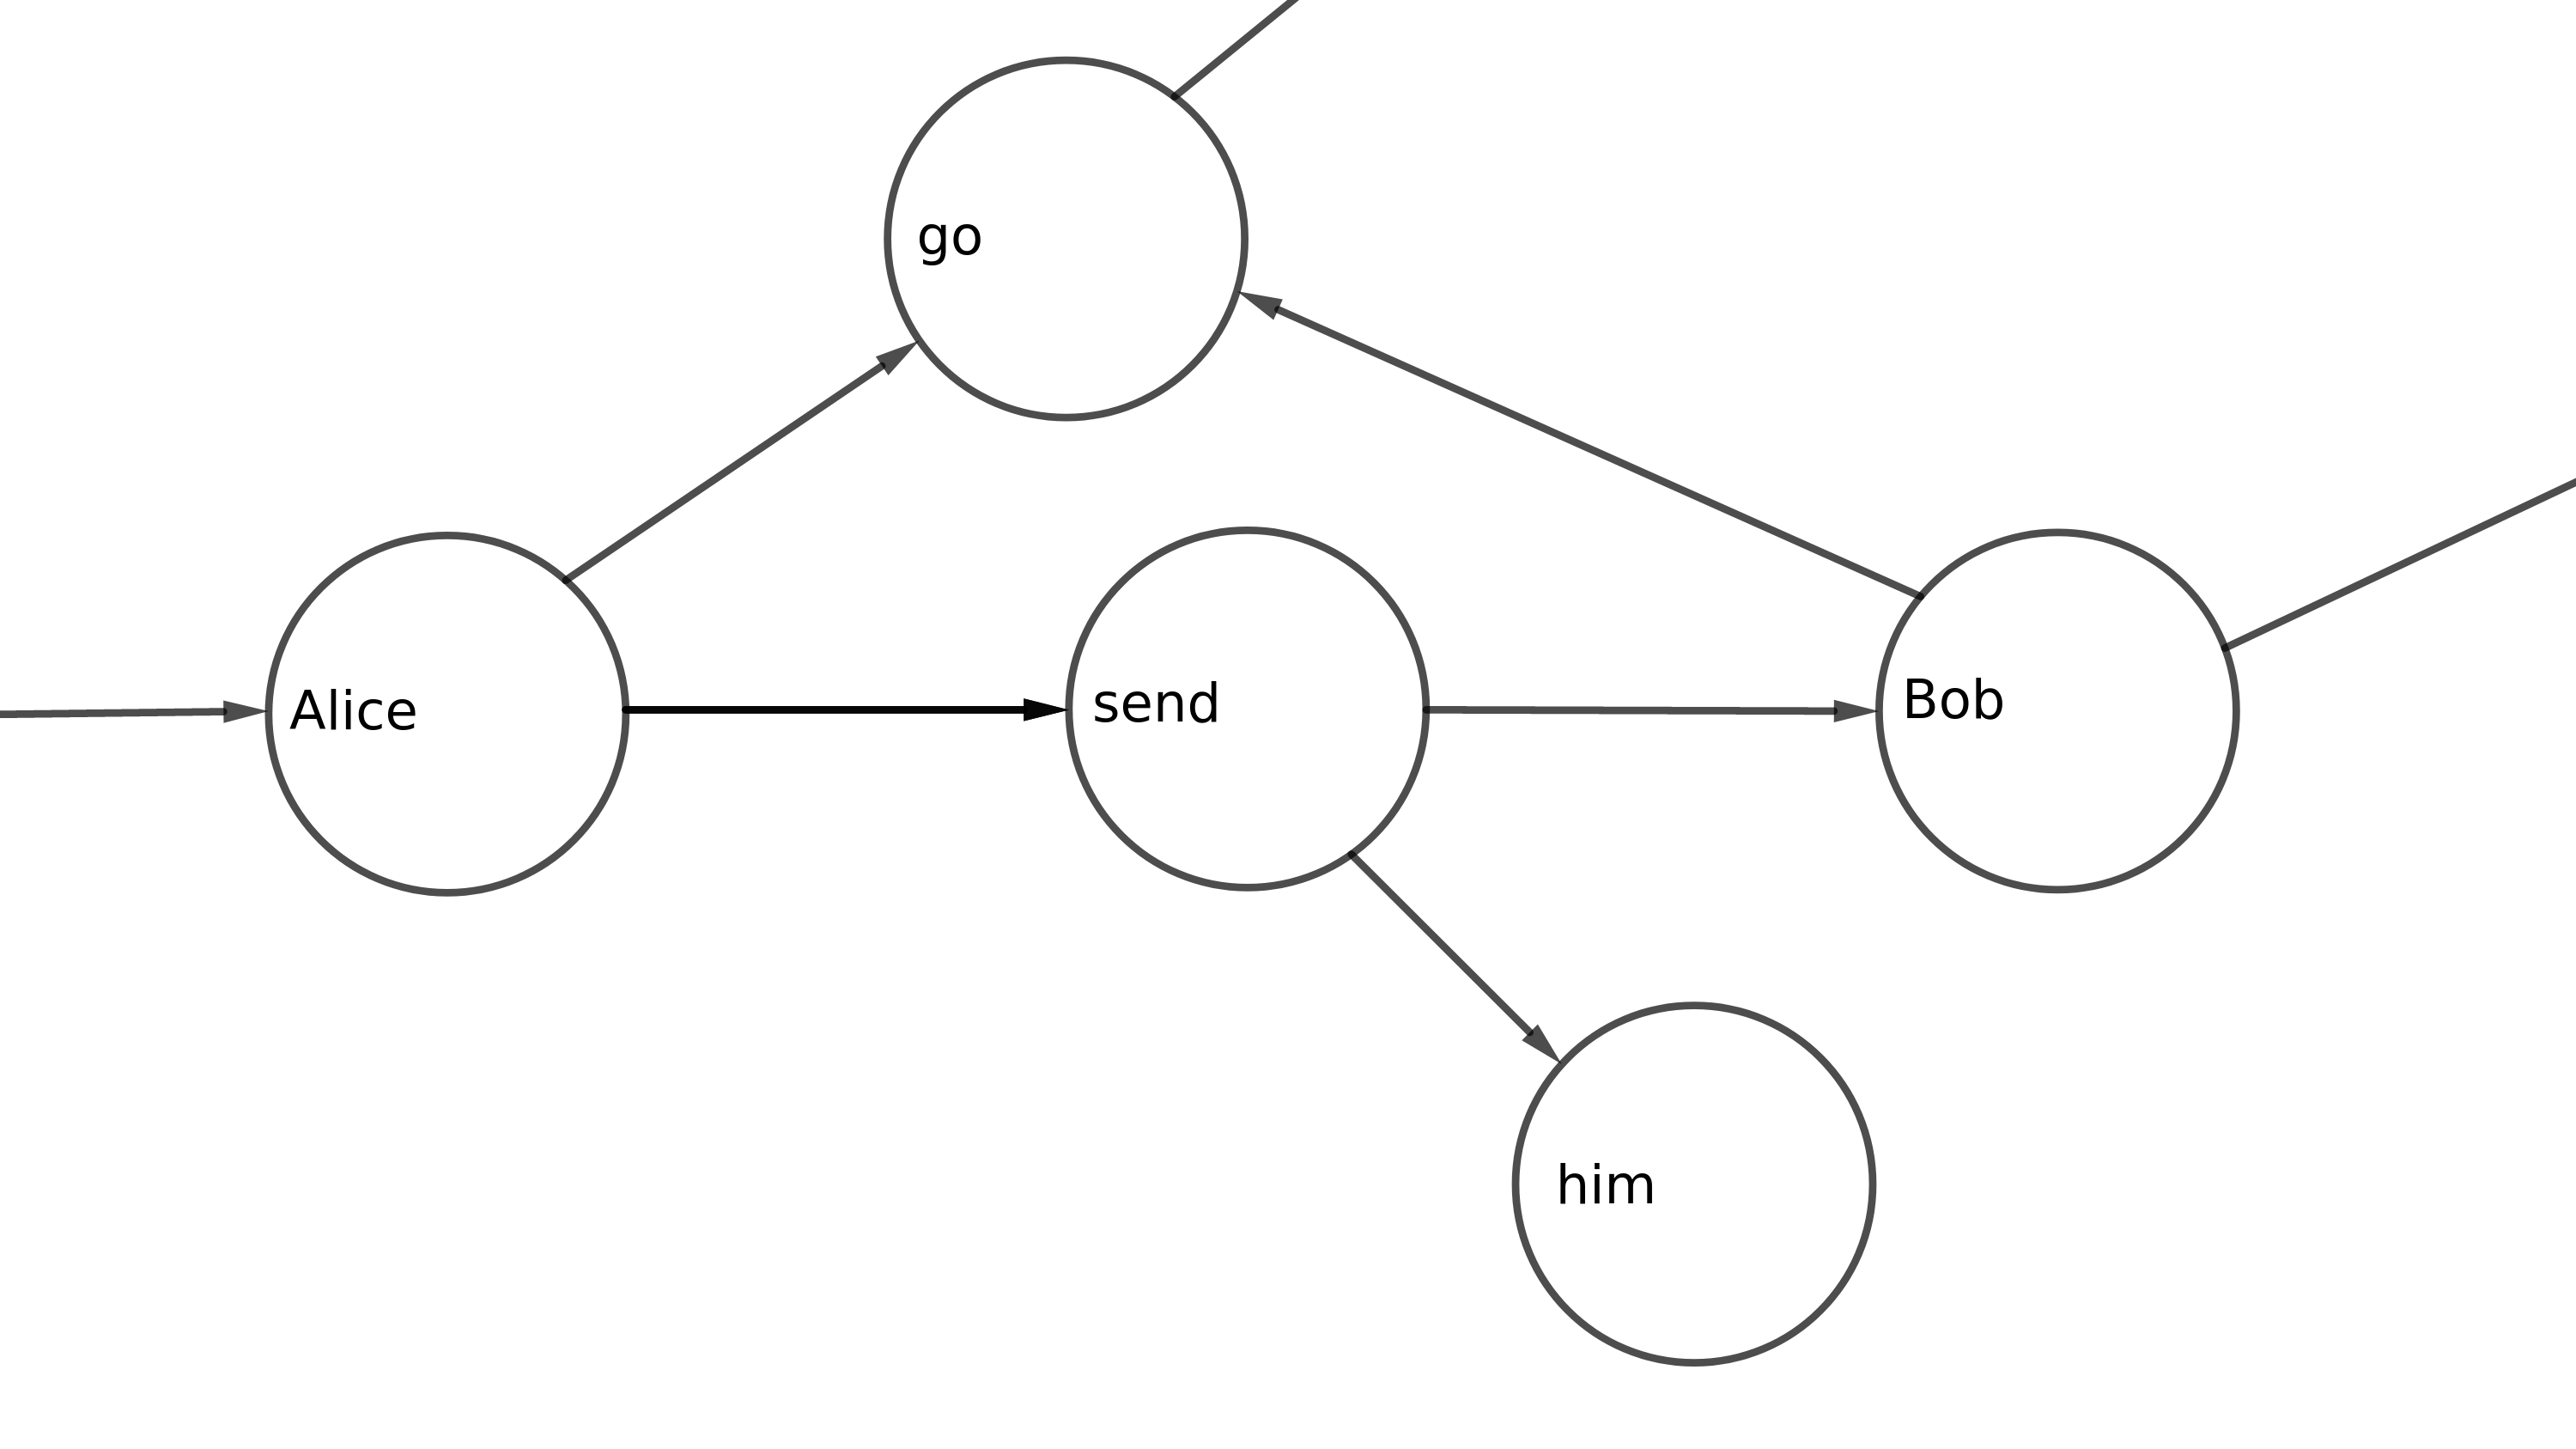
\includegraphics[scale=0.39]{Bilder/w2w_big}
			\end{figure}
		\end{column}
	\end{columns}
% --------------------------------------
\mynote{
	\begin{itemize}
		\item In the next steps more and more rules are added
	\end{itemize}
}
\end{frame}

% === OHE AND W2V ===================================

\begin{frame}
\frametitle{Word to word flavors}
\framesubtitle{\onehot{s} \& Word vectors}
	\begin{itemize}
		\item<1-> Word to word models come in two flavors
		\begin{itemize}
			\item<2-> \onehot{s} and
			\item<3-> Word vectors
			\item[] % Direkt einblenden, damit man nicht 2-3x weiterklicken muss
		\end{itemize}
	\end{itemize}
	\begin{columns}
		% SPALTE 1
		\begin{column}{0.375\textwidth}
			\begin{itemize}[leftmargin=15mm]
				\item<4-> Are $ 300d $ real valued vectors
				\item<5-> Potentially incorporate more information about a word
				\begin{itemize}
					\item<6->[$ \Rightarrow $] Better learning possible?
				\end{itemize}
				\item<7-> Probably the hippocampus receives multiple signals which are in total more related to word vector than to \onehot{}
				\begin{itemize}
					\item<8->[$ \Rightarrow $] Closer to reality
				\end{itemize}
			\end{itemize}
		\end{column}
		% SPALTE 2
		\begin{column}{0.625\textwidth}
			\begin{figure}
                \begin{overprint}
                    \centering
                        \includegraphics<1>[scale=0.39]{Bilder/w2w_big}
                        \includegraphics<2>[scale=0.39]{Bilder/w2w_ohe_big}
                        \includegraphics<3->[scale=0.39]{Bilder/w2w_w2v_big}
                \end{overprint}
			\end{figure}
		\end{column}
	\end{columns}
\mynote{
\begin{itemize}
    \item[ü] KEINE ÜBERLEITUNG
    \item word to word models come in two flavors
    \begin{itemize}
        \item equipped with \onehot{s} and ...
        \item word vectors
    \end{itemize}
	\item Word vectors can be calculated with \texttt{spacy} and are $ 300d $ real valued vectores as indicated in the graph
	\item They potentially incorporate more information about a word, STICHPUNKT EINBLENDEN therefore we hope they increase learning quality.
	\item Probably the hippocampus receives multiple signals which are in total more related to word vector than to \onehot{} STICHPUNKT EINBLENDEN
\end{itemize}
}
\end{frame}

% === AVERAGE APPROACH ===================================

% TODO Die anderen Konfigurationen erwähnen, am besten auf neue Folie
\begin{frame}[label={frame: average approach}]{Word to word Models}{Average approach}
	\begin{itemize}
		\item<+-> Predicting all instances of a word class at once and average the result (into one vector)
		\item<+-> Word classes are inferred by {\huge \texttt{spacy}}, $ 10 $ in total are used
		\item<+-> Idea: Meta word pairs like {\huge \texttt{Pronoun → Verb}} appear more frequently than {\huge \texttt{he → plays}}
		\item<+-> Averaging is done with both vector types: \onehot{s} and word vectors
	\end{itemize}
% --------------------------------------
\mynote{
\begin{itemize}
    \item[ü] There is also an average approach for word to word models
	\item It works by predicting all instances of a word class at once and average the result (into one vector)
	\item The word classes of the $ 10 $ highest indices are inferred by {\huge \texttt{spacy}}
	\item The idea behind averaging was that meta word pairs like {\huge \texttt{Pronoun → Verb  (Pronoun followed by Verb)}} appear more frequently than {\huge \texttt{he → plays (he then plays)}}, so a coarser tool may be worth trying
	\item The Averaging takes place for both vector types: \onehot{s} and word vectors
\end{itemize}
}
\end{frame}

\chapter{Methodology and Results} \label{ch: results}

% ======================================

\section{First Model and Architecture} \label{sec: first model and architecture MR}
The predefined structures, as they were mentioned in \secreff{subsec: first model and architecture}, form the base of these model types \ie a rule set was given which is equivalent to a graphical model, where the rules describe the edges. The training data was composed by randomly choosing one of the five rules and the input as well as the output word. The Neural Network was quite shallow because it contained only one hidden layer.
By using eight words from each class, the rules are easily learned (\figref{\ref{fig: first model tpm and mds}}).
\begin{figure}
	\centering
		\subcaptionbox{Learned Successor Representation of a tailored \cognitiveroom{} with apparent future states.}{
			\includegraphics[height=\twocolpicheight]{chapter4/chapter4.1/first_models/4Rules/plots/First Model + More Rules_100E_100BS_1L_1C/Transition_Probability_Matrix;_t=1,_DF=0.5.png}
		}
		\hfill
		\subcaptionbox{\gls{mds} plot of the \gls{sr} in (a) showing decent clusters.}{
			\includegraphics[height=\twocolpicheight]{chapter4/chapter4.1/first_models/4Rules/plots/First Model + More Rules_100E_100BS_1L_1C/MDS_of_Transition_Probability_Matrix;_t=1,_DF=0.5.png}
		}
	\caption{Clearly visible are the successor positions of the states \eg \texttt{Adjective → Noun}. \texttt{Nouns} are smeary because the rule set in \secreff{enum: rule set} doesn't provide one starting with \texttt{Noun}, so the Neural Network has to guess in less definite scenarios. Although there is a prediction made for each single word \ie state in the \cognitiveroom{}, only word classes are displayed to avoid clutter (Pers. Pr. = \texttt{Personal Pronoun}, Pos. Pr. = \texttt{Possessive Pronoun}).}
	\label{fig: first model tpm and mds}
\end{figure}
Since the rows encode the states, it is expected in the terms of the successor representation that the next position shows a high activation. Checking this behavior is simple because the environment (\secreff{subsec: first model and architecture}) is clearly defined. The \texttt{Noun} part of \figref{\ref{fig: first model tpm and mds}} is smeary because there is no rule for a consecutive state (in graph theory it corresponds to a sink). The undefined behavior is also revealed in the \gls{mds} illustration, where all nouns are distributed between the other word classes. By calculating the \gls{sr} for additional time steps, the result incorporates all following rules or states (\figref{\ref{fig: first model sr t=3, df=0.5}}). These matrices are interesting for analyzing the value function $ V $ (\equref{\eqref{eq: v with sr-matrix}}), which is beyond the scope of this work.
\begin{figure}
	\centering
		\subcaptionbox{Calculated \gls{sr} of a tailored \cognitiveroom{} for $ t = 2 $ and $ \gamma = 0.5 $ using the matrix of \figref{\ref{fig: first model tpm and mds}}.}{
			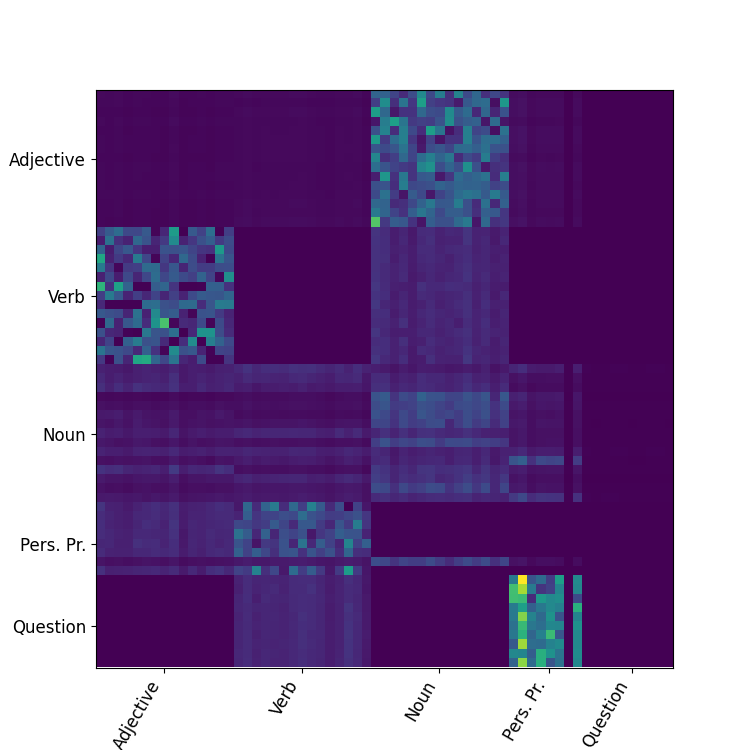
\includegraphics[height=\twocolpicheight]{chapter4/chapter4.1/first_models/4Rules/plots/First Model + More Rules_100E_100BS_1L_1C/SR,_t=2,_DF=0.5.png}
		}
		\hfill
		\subcaptionbox{\gls{mds} plot of the \gls{sr} in (a) with properly grouped word classes}{
			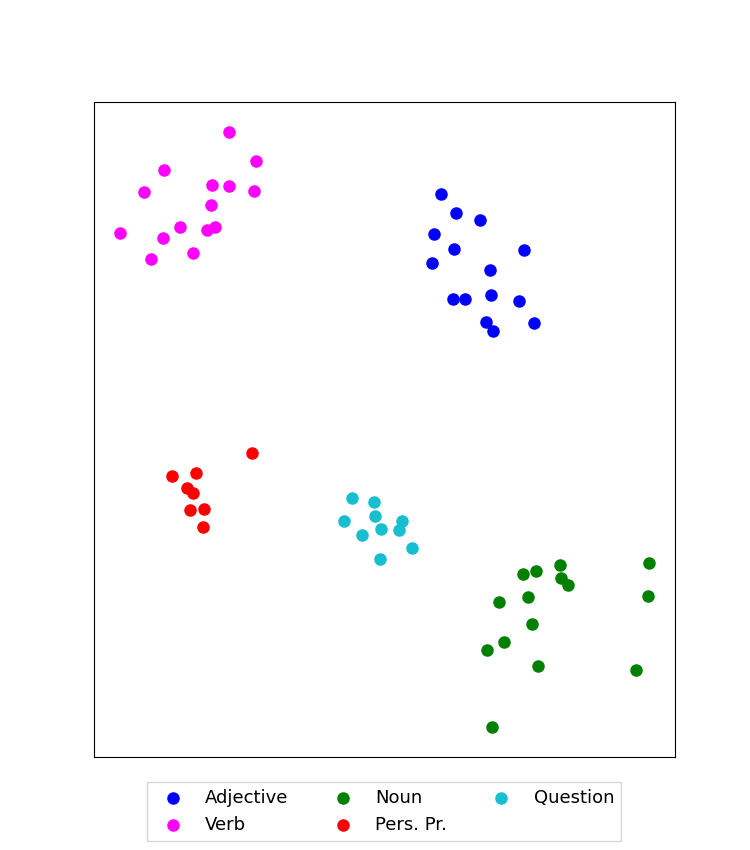
\includegraphics[height=\twocolpicheight]{chapter4/chapter4.1/first_models/4Rules/plots/First Model + More Rules_100E_100BS_1L_1C/MDS_of_SR,_t=2,_DF=0.5.png}
		}
	\caption{Calculating the Successor Representation for a higher time step \ie $ t=2 $, already demonstrates the properties of the construction. For all states (visual aggregated into the word class), it is possible to derive successor states \eg the two step rule \texttt{Question → Pers. Pr. → Verb}.}
	\label{fig: first model sr t=3, df=0.5}
\end{figure}
%The \gls{sr} doesn't serve the purpose of predicting future states because then the plot in \figref{} would be misleading. In this case it suggests staying in the \texttt{Pronoun} state after $ t = 3 $ which is impossible because pausing \eg \texttt{Pronoun → Pronoun} is no valid rule. And also reentering the state after leaving it is no option since \texttt{Question} is the single possibility for transiting \texttt{Pronoun} but \texttt{Question} has no predecessor. The \gls{sr} has to be read in terms of the value function $ V $ in \eqref{eq: v with sr-matrix}.

\bigskip
% \TODOL{Aufzählung im Moment aufgeteilt, muss nicht sein. Evtl. doch wieder in den Fließtext.}
The principle also works out when using more rules and a larger data set. The enhancement is done by introducing four new rules
\begin{itemize}
	\item \texttt{Question word → Verb}
	\item \texttt{Noun → Personal Pronoun}
	\item \texttt{Adverb → Possessive Pronoun}
	\item \texttt{Personal Pronoun → Adverb},
\end{itemize}
more words for the already existing categories and two new word classes (\texttt{Adverb} and \texttt{Possessive Pronoun}). The result in \figref{\ref{fig: more rules and word tpm and mds}} is in clarity similar to \figref{\ref{fig: first model tpm and mds}} but without having an obvious blurry row, even though the word class \texttt{Possessive Pronoun} is without successor as \texttt{Noun} in the trial before. Nevertheless, some similarities to \texttt{Question word} were detected. The only characteristic they seem to share is having exactly one edge. Also, clusters are in the \gls{mds} apparent, indicating learning worked. Although artificial, conceptually they serve as a standard to reach for the upcoming configurations.
\begin{figure}
	\centering
		\subcaptionbox{\gls{sr} of a more advanced model.}{
			\includegraphics[height=0.375\textheight]{chapter4/chapter4.1/first_models/8Rules/plots/First Model + More Rules_100E_100BS_1L_1C/Transition_Probability_Matrix;_t=1,_DF=0.5.png}
		}
		\hfill
		\subcaptionbox{\gls{mds} plot of (a).}{
			\includegraphics[height=0.375\textheight]{chapter4/chapter4.1/first_models/8Rules/plots/First Model + More Rules_100E_100BS_1L_1C/MDS_of_Transition_Probability_Matrix;_t=1,_DF=0.5.png}
		}
	\caption{The illustrated plots stem from a model using additional rules backed by more word classes and a larger database to retrieve the training data. The outcomes are similar to \figref{\ref{fig: first model tpm and mds}}. The upcoming states are obvious. The model can handle ambiguous successors \eg \texttt{Personal Pronoun → Verb} and \texttt{Personal Pronoun → Adverb} are deployed rules.}
%		Learned Successor Representation (left) and corresponding \gls{mds} plot (right) of a more advanced model consisting of eight rules backed by a larger variety of words used for training.}
	\label{fig: more rules and word tpm and mds}
\end{figure}


% ======================================

\section{Word to word models} \label{sec: text based models and architecture}
The harder challenge lies in processing natural languages. For this purpose two different approaches, namely the \nameref{subsubsec: onehot approach} and the \nameref{subsubsec: word vector approach} were examined. The ambitious goal was to learn or get a sense of the grammatical structure of the text. In practice, this means that after feeding \eg an adjective into the Neural Network, it should propose words or word classes which follow this word.
%Since the book is written in german, \texttt{Nouns} and \texttt{Adjectives} are obvious candidates for a successor but since it's free word order it is not possible to rely on these word classes since german has a variable word order\TODO{Vllt. ausführlicher schildern und/oder Referenz im Todo-Kommentar der tex-Datei hinzufügen}.
%% TODO https://en.wikipedia.org/wiki/V2_word_order#Examples_of_verb_second_(V2)
In the following paragraphs an schematic outline of the model will be given \ie few data was involved to achieve more reasonable diagrams. The full book covers multiple thousands of states, leading to a sparse squared matrix in this dimension. Thus, depicting matrices no longer makes sense.

To be able to evaluate the results, a ground truth distribution was calculated for gaining a qualitative and quantitative measure (\figref{\ref{fig: text model gt}}). The data set is labeled on the axes. There is also a \gls{mds} plot next to it because on large scale models ($ > 500 $ words) it is impossible to get visual feedback just by inspecting the matrix plot. The hope is that clusters of the same color appear as in \secreff{sec: first model and architecture MR}, because meta word pairs, for example \texttt{Noun → Verb} \eg \texttt{Alice → goes} and \texttt{wood → breaks}, should share some features and be mapped close to each other. Furthermore, similarities are to some extent also visible by looking at the \gls{mds}.

Having a reference now, the model was set up for training. In \figref{\ref{fig: text model sr}} is an emblematic transition matrix illustrated. Whereas in \secreff{sec: first model and architecture MR}, it was easy to recognize the rules in the \gls{sr}, this will no longer be possible due to the sheer amount of states. Hence, the cluster plot is more important to gain visual intuition for the results.
%
\begin{figure}
	\centering
		\subcaptionbox{Examplary ground truth distribution of a tiny data set.}{
		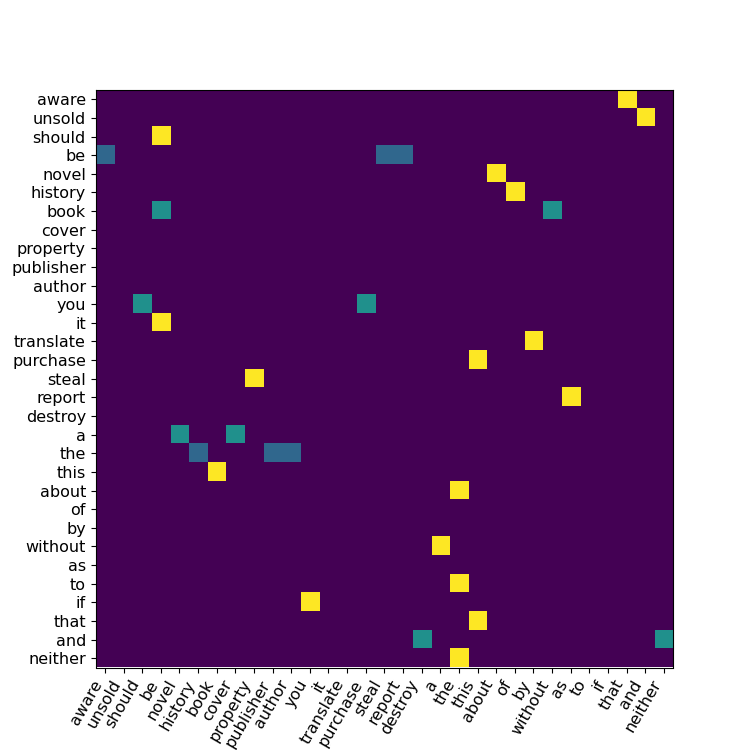
\includegraphics[height=\twocolpicheight]{Bilder/chapter4/BspW2W/plots/OHE_OHE_500E_100BS_1L_1C_5P_30T_J/J_5pages_30T_words.png}
	}
		\hfill
		\subcaptionbox{Corresponding \gls{mds} plot of the ground truth in (a).}{
			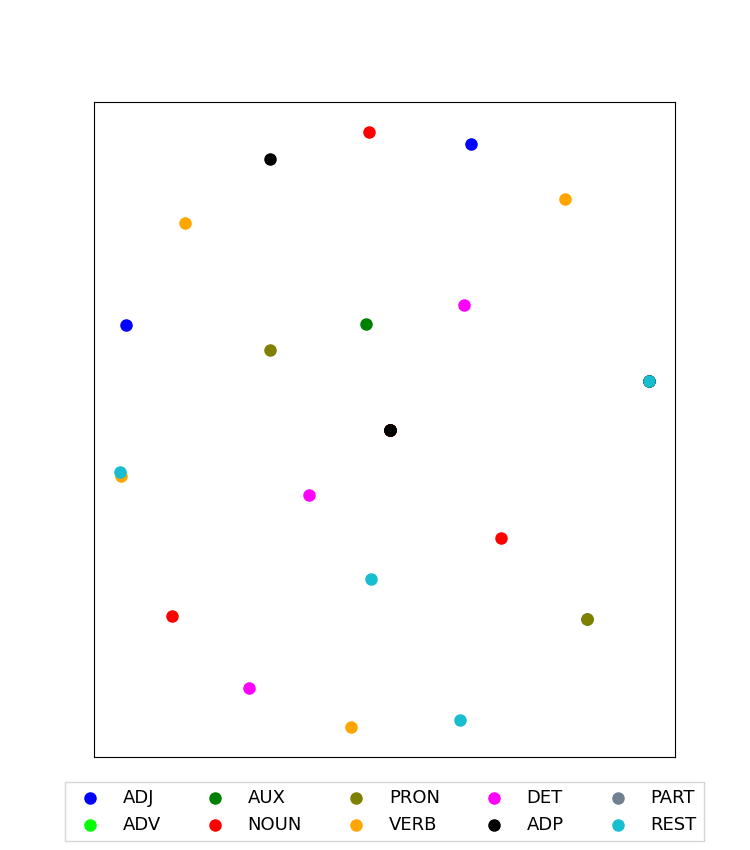
\includegraphics[height=\twocolpicheight]{Bilder/chapter4/BspW2W/plots/OHE_OHE_500E_100BS_1L_1C_5P_30T_J/MDS_J_5pages_30T_words.png}
		}
	\caption{For illustrative purposes only a tiny data set \ie few words of the book were processed to calculate the ground truth distribution.}
	\label{fig: text model gt}
\end{figure}
%
\begin{figure}
	\centering
		\subcaptionbox{Learned \srmat{} of model using \onehot{s} during training.}{
			\includegraphics[height=\twocolpicheight]{chapter4/BspW2W/plots/OHE_OHE_500E_100BS_1L_1C_5P_30T_J/Transition_Probability_Matrix;_t=1,_DF=0.5.png}
		}
		\hfill
		\subcaptionbox{\gls{mds} clustering of the Successor Representation in (a).}{
			\includegraphics[height=\twocolpicheight]{chapter4/BspW2W/plots/OHE_OHE_500E_100BS_1L_1C_5P_30T_J/MDS_of_Transition_Probability_Matrix;_t=1,_DF=0.5.png}
		}
	\caption{Transition probability matrix of a model using constructed rules by processing a book and \onehot{s} during training. Hence, the environment is no longer manufactured. Whereas the results of the models in \secreff{sec: first model and architecture MR} were fully described by the matrix plot, this will no longer be possible for large scale models because the matrix becomes to huge. As seen before, the \gls{mds} can occupy this role. If sufficient learning happened, clusters or similarities to the corresponding plot of the ground truth should be recognizable. (Though not when illustrating with the tiny data set.)}
	\label{fig: text model sr}
\end{figure}

% --------------------------------------

\subsection{Word to word models: Evaluating the results} \label{subsec: text model evaluating the results}
To achieve the best result, four configurations were tested and compared in \tabref{\ref{tab: text model versions and metrics}} by the metric introduced in \secreff{sec: metric}.
\begin{table}
	\centering
	\caption{Trained models with metric values regarding their corresponding ground truth. ``german'' and ``english'' refer to the book which provided the data set (s. \secreff{sec: data preparation}). The associated \gls{mds} plots for a qualitative feedback can be found in \figref{\ref{fig: text model gt de en mds}} and \figref{\ref{fig: text model cumulativ mds plots}} of \appref{ch: appendix text model}.}
	\begin{tabular}{ll}
		\toprule
		Version					& Metric \\
		\midrule
		german, \onehot{} 		& $ 0.08 $	\\% 0.08200
		german, word vector		& $ 0.74 $	\\% 0.74139
		english, \onehot{}		& $ 0.10 $	\\% 0.10021
		english, word vector	& $ 0.78 $	\\% 0.77522
		\bottomrule
	\end{tabular}
	\label{tab: text model versions and metrics}
\end{table}
Surprisingly, the german and english \onehot{} versions nearly don't differ. Not only regarding the model used to collect the data but in general. Due to the beforehand mentioned freer word order german incorporates, a better score for the english based models was expected.

It is obvious that the models using word vectors perform quite bad compared to the \onehot{} variants. The reason may be on one hand that language is a structural complex field and on the other that too many uncertainties are attached to word vectors. Learning is more difficult since $ 300 $ distinct values are involved, whereas a \onehot{} may be quite accurate if the learned version has its maximum near or at the index where the input vector is equal to $ 1 $. Also back-calculating the output to a word is a process of compromises because it is guaranteed that \spacy{} doesn't provide a word vector with the exact same components and it is necessary to limit on the $ n $ closest word vectors/words. The disappointing outcome of the word vector model is furthermore frustrating since it is more probable that the hippocampus doesn't process signals which are close to \onehot{s} (or an analogy of it) but rather multiple stimuli decoding different characteristics, thus more related to a word vector.

\paragraph{Additional configurations}
While searching for the best parameters, not just the four versions mentioned were examined. Most of the time was consumed by finding a promising setup. This is reflected by some parameters the framework provides (\eg \texttt{nmb\_hidden\_layers}, \secreff{ap: parameters}), which aren't necessary to reproduce the results presented in this work. A subset with illustrations and short documentation of all variants can be found in \appref{ch: additional configurations}.

% --------------------------------------

%%%\subsection{Additional configurations} \label{subsec: additional configurations}
%To draw a full picture, plenty of approaches which had the goal to improve the results will be mentioned in this chapter. Sadly, no one changed the outcome by any means. Facing this presented an enormous obstacle while researching. Some of them will be presented shortly in this chapter. In all cases it is obvious that these configurations were dead ends.
%
%The architectures included
%\begin{itemize}
%	\item different number of epochs from $ 100 $ to $ 50000 $
%	\item $ 2 $-hot-encoded vectors
%	\item an auto-encoder structure
%\end{itemize}
%
%% --------------------------------------
%
%\section{Multiple hidden layers} \label{subsubsec: multiple hidden layers}
%Different numbers of layers ranging from $ 1 $ to $ 100 $ were tested, some example results will be depicted. 
%\begin{figure}[H]
%	\centering
%	\subcaptionbox{\gls{sr} of a model using english and \onehot{s} with $ 40 $ hidden layers.}{
%		\includegraphics[height=\twocolpicheight]{Bilder/chapter4/additional_configurations/OHE_OHE_4000E_100BS_40L_1C_200P_1500T_J/Transition_Probability_Matrix;_t=1,_DF=0.5.png}
%	}
%	\hfill
%	\subcaptionbox{\gls{mds} of the matrix in (a).}{
%		\includegraphics[height=\twocolpicheight]{Bilder/chapter4/additional_configurations/OHE_OHE_4000E_100BS_40L_1C_200P_1500T_J/MDS_of_Transition_Probability_Matrix;_t=1,_DF=0.5.png}
%	}
%	\caption{Although mentioned that transition probability matrices don't show anything if too many words are used, they can be used sometimes to detect failure. The reference, at least for the \gls{mds}, is illustrated in \figref{\ref{fig: w2w model gt en}}. The value of the metric is $ 0.50 $, the equivalent with one layer achieves $ 0.10 $ (s. \tabref{\ref{tab: text model versions and metrics}} to get a full list). This could imply that more layers hamper learning.}
%	\label{fig: text model en ohe 40L}
%\end{figure}
%%
%\begin{figure}[H]
%	\centering
%		\subcaptionbox{\gls{mds} of a model using english and \onehot{s} with $ 2 $ hidden layers.}{
%			\includegraphics[height=\twocolpicheight]{Bilder/chapter4/additional_configurations/OHE_OHE_4000E_100BS_2L_1C_200P_1500T_J/MDS_of_Transition_Probability_Matrix;_t=1,_DF=0.5.png}
%		}
%		\hfill
%		\subcaptionbox{\gls{sr} of a model using english and \onehot{s} with $ 10 $ hidden layers.}{
%			\includegraphics[height=\twocolpicheight]{Bilder/chapter4/additional_configurations/OHE_OHE_7000E_100BS_10L_1C_200P_1500T_J/Transition_Probability_Matrix;_t=1,_DF=0.5.png}
%		}
%	\caption{As mentioned before, more layers result in worse \glspl{sr}. Already one additional hidden layer lowers the metric. The model in (a) reaches $ 0.22 $, whereas with one hidden layer the value is $ 0.10 $. The network in (b) was configured with $ 10 $ hidden layers and the successor representation looks indistinguishable from one training with $ 40 $ (\figref{\ref{fig: text model en ohe 40L}}).}
%\end{figure}
%
%% --------------------------------------
%
%\section{Many epochs combined with multiple hidden layers}
%The example outputs stem from a model which trained with sixfold epochs and $ 40 $ hidden layers.
%\begin{figure}[H]
%	\centering
%		\subcaptionbox{English, \onehot{s}, $ 25,000 $ epochs and $ 40 $ layers.}{
%			\includegraphics[height=\twocolpicheight]{Bilder/chapter4/additional_configurations/OHE_OHE_25000E_100BS_40L_1C_200P_1500T_J/Transition_Probability_Matrix;_t=1,_DF=0.5.png}
%		}
%		\hfill
%		\subcaptionbox{\gls{mds} of a model using english, word vectors, $ 25,000 $ epochs and $ 40 $ layers}{
%			\includegraphics[height=\twocolpicheight]{Bilder/chapter4/additional_configurations/W2V_W2V_25000E_100BS_40L_1C_200P_1500T_J/MDS_of_Transition_Probability_Matrix;_t=1,_DF=0.5.png}
%		}
%	\caption{The only conclusion to draw from this plot of two different models is that additional epochs might lead to a full degeneration of the results if word vectors are used for training. The \onehot{} analogue shows no mismatch to them of \secreff{subsubsec: multiple hidden layers}.}
%\end{figure}
%
%% --------------------------------------
%
%\section{Using word vectors to learn an \onehot{}}
%This configuration is combination of two mainly used in the thesis. It uses word vectors as input and \onehot{s} as output \ie it uses heterogeneous structured training data.
%\begin{figure}[H]
%	\centering
%		\subcaptionbox{English, word vector to \onehot{} as \gls{mds}.}{
%			\includegraphics[width=\twocolpicwidth]{Bilder/chapter4/additional_configurations/W2V_OHE_5000E_100BS_1L_1C_200P_1500T_D/MDS_of_Transition_Probability_Matrix;_t=1,_DF=0.5.png}
%		}
%	\hfill
%		\subcaptionbox{German, ground truth \gls{mds} of word to word transitions.}{
%			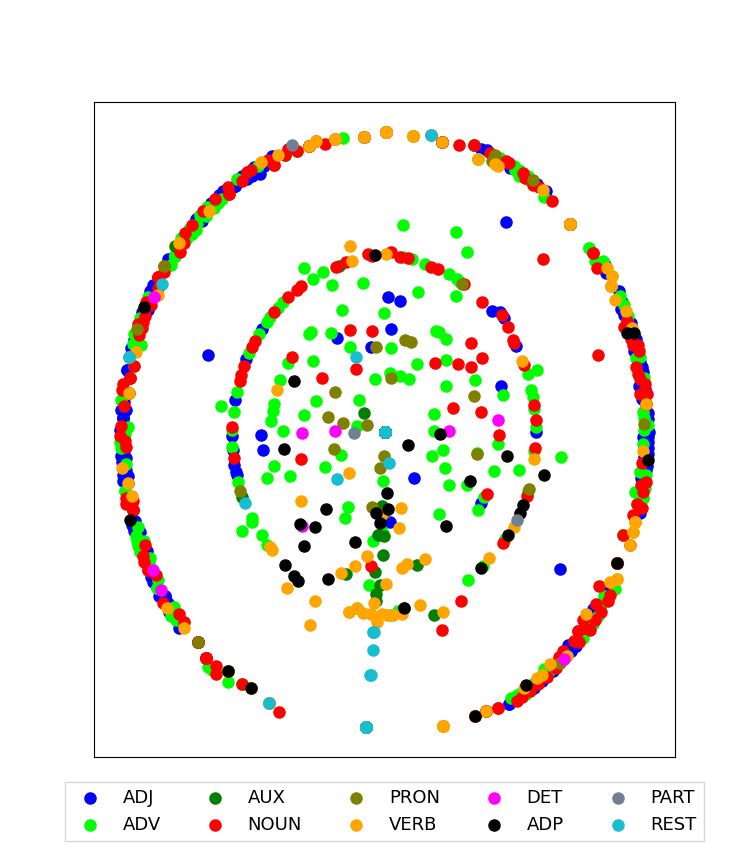
\includegraphics[width=\twocolpicwidth]{Bilder/chapter4/W2W/ground_truths/MDS_D_200pages_1500T_words.png}
%		}
%	\caption{\gls{mds} plot of a model using german training data and word vectors as input to learn a \onehot{}. The results lack characteristics to draw sensible conclusions from. Though it is possible to calculate the metric for the configuration: $ 0.47 $. By comparing with \tabref{\ref{tab: text model versions and metrics}}, it sits between its full \onehot{} and word vector relatives.}
%\end{figure}
%
%% --------------------------------------
%
%\section{Multiplying the training data} \label{subsubsec: multiplying training data}
%The goal of multiplying the training data \ie concatenating the training data $ n $ times with itself, was to have the opportunity to see the training data more often during one epoch.
%\begin{figure}[H]
%	\centering
%		\subcaptionbox{German, \onehot{s} with $ 5 $ concatenations.}{
%			\includegraphics[width=\twocolpicwidth]{Bilder/chapter4/additional_configurations/OHE_OHE_5000E_100BS_1L_5C_200P_1500T_D/MDS_of_Transition_Probability_Matrix;_t=1,_DF=0.5.png}
%		}
%		\hfill
%		\subcaptionbox{German, word vectors with $ 5 $ concatenations.}{
%			\includegraphics[width=\twocolpicwidth]{Bilder/chapter4/additional_configurations/W2V_W2V_5000E_100BS_1L_5C_200P_1500T_D/MDS_of_Transition_Probability_Matrix;_t=1,_DF=0.5.png}
%		}
%	\caption{Concatenating the training data $ 5 $ times with itself doesn't change outcomes (compare \figref{\ref{fig: text model cumulativ mds plots}}). This impression is fortified by the metrics both models achieve: $ 0.14 $ for \onehot{s} and $ 0.72 $ with word vectors ($ 0.08 $ and $ 0.74 $ without respectively, \tabref{\ref{tab: text model versions and metrics}}).}
%\end{figure}
%
%% --------------------------------------
%
%\section{Calculating high time steps}
%One idea was to calculate high time steps of the \gls{sr} hoping the irregularities even out in distant future.
%\begin{figure}[H]
%	\centering
%		\subcaptionbox{\gls{mds} of a \gls{sr} with $ t = 20 $. German and \onehot{s} were used during training.}{
%			\includegraphics[width=\twocolpicwidth]{Bilder/chapter4/additional_configurations/hohes_t/OHE_OHE_5000E_100BS_1L_1C_200P_1500T_D/MDS_of_SR,_t=20,_DF=0.5.png}
%		}
%		\hfill
%		\subcaptionbox{\gls{mds} of a \gls{sr} with $ t = 50 $. German and \onehot{s} were used during training.}{
%			\includegraphics[width=\twocolpicwidth]{Bilder/chapter4/additional_configurations/hohes_t/OHE_OHE_5000E_100BS_1L_1C_200P_1500T_D/MDS_of_SR,_t=50,_DF=0.5.png}
%		}
%	\caption{High times also don't bring progress since no evident structure is recognizable within the plots. A comparison with the ground truth wouldn't bring additional insights too because the underlying matrices can't be interpreted as transition probability matrices.}
%	\label{fig: high time steps ohe}
%\end{figure}
%%
%\begin{figure}[H]
%	\centering
%		\subcaptionbox{\gls{mds} of a \gls{sr} with $ t = 20 $. German and word vectors were used during training.}{
%			\includegraphics[width=\twocolpicwidth]{Bilder/chapter4/additional_configurations/hohes_t/W2V_W2V_5000E_100BS_1L_1C_200P_1500T_D/MDS_of_SR,_t=20,_DF=0.5.png}
%		}
%		\hfill
%		\subcaptionbox{\gls{mds} of a \gls{sr} with $ t = 50 $. German and word vectors were used during training.}{
%			\includegraphics[width=\twocolpicwidth]{Bilder/chapter4/additional_configurations/hohes_t/W2V_W2V_5000E_100BS_1L_1C_200P_1500T_D/MDS_of_SR,_t=50,_DF=0.5.png}
%		}
%	\caption{As before in \figref{\ref{fig: high time steps ohe}} no structure is recognizable to do further research on. Results relying on word vectors again seem to be very labile and degenerate.}
%\end{figure}
%
%% --------------------------------------
%
%\section{Predict only the most frequent words}
%Similar to \secreff{subsubsec: multiplying training data}, the most frequent words of the text are seen more often by the network. Hence it might be able to learn these inputs better than ordinary ones.
%\begin{figure}[H]
%	\centering
%		\subcaptionbox{German with word vectors. \gls{mds} of the $ 40 $ most frequent words.}{
%			\includegraphics[width=\twocolpicwidth]{Bilder/chapter4/additional_configurations/MostFrequentWords_4000E_100BS_1L_1C_200P_1500T_D/MDS_of_Transition_Probability_Matrix;_t=1,_DF=0.5.png}
%		}
%		\hfill
%		\subcaptionbox{Same \gls{mds} plot as in (a) but annotated with \postag{s}instead of words.}{
%			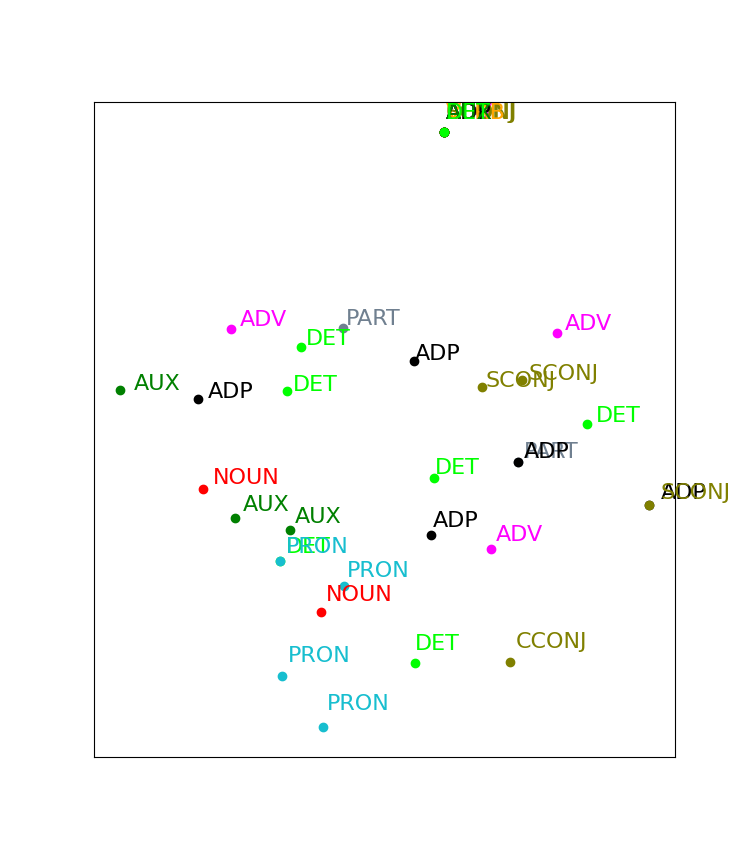
\includegraphics[width=\twocolpicwidth]{Bilder/chapter4/additional_configurations/MostFrequentWords_4000E_100BS_1L_1C_200P_1500T_D/ud_pos_tag_annotated.png}
%		}
%	\caption{The same model with german data set and word vectors as in \secreff{sec: text based models and architecture} was trained. Predictions were limited to the $ 40 $ most frequent words. For a better overview the second plot was labeled with the corresponding \postag{s}.}
%\end{figure}


%The ambitions goal of detecting grammatical rules by using encoded words as \onehot{} or word vector wasn't achieved by solely evaluating the plain word models.


% ======================================

\section{Averaging models} \label{sec: average approach}
Because large scale word to word models seem to lack characteristics for a proper evaluation and interpretation of the results, the average approach was developed (\secreff{subsubsec: average approach}). The main idea is to rearrange the output of the formerly presented models, because general patterns like \texttt{Noun → Verb} or \texttt{Determiner → Adjective} appear significantly more frequently than certain instances as \texttt{sun → shines} or \texttt{an → old}. By averaging the predictions, one might be able to catch the structure in general.

Since \secreff{subsubsec: average approach} only provided a rough description of the principle, it shall be extended in the following. After the collective prediction of one word class, all outputs are averaged having one vector resembling the complete data in the dimension of the \cognitiveroom{} containing the associated frequencies. In the next step the $ n $ indices (in practice $ 10 $ was used) with the highest values are checked for their \postag{}. So, if index $ i $ is one of these and encodes the word \texttt{fish}, its \postag{} \ie \texttt{NOUN} is counted. Finally, a vector is constructed for all word classes where each component resembles the probability for the successor word class. Some final numbers are illustrated in \figref{\ref{fig: barplot det adp}}.

To get an idea of the learned results, some valid sentences are provided in German (the language of the training data of \figref{\ref{fig: barplot det adp}}) in \tabref{\ref{tab: example sentences}}. This short sanity check implies that no cacophony is learned and the outputs are reasonable.
\begin{figure}
	\centering
		\subcaptionbox{Averaged transitions of all \texttt{ADP}s compared to the ground truth.}{
			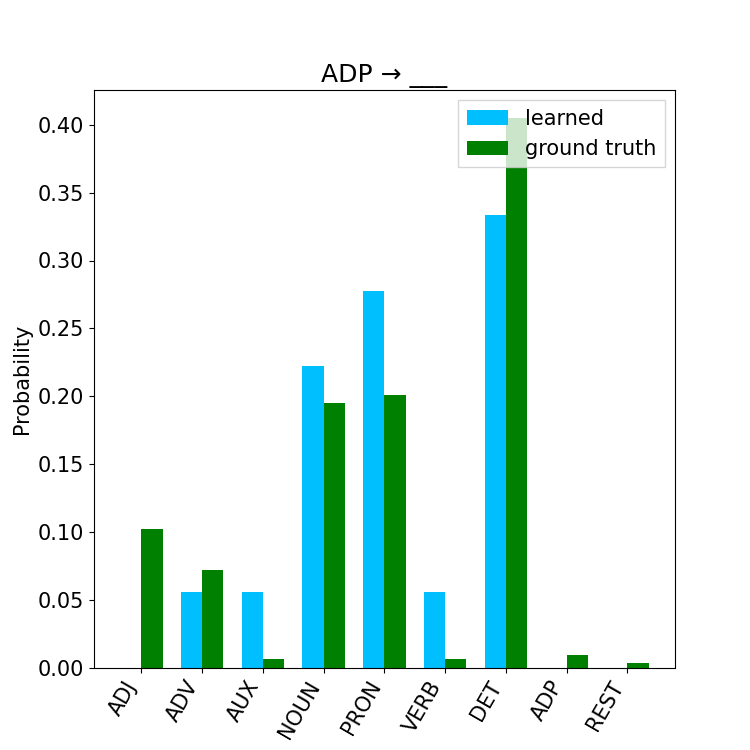
\includegraphics[width=\twocolpicwidth]{Bilder/chapter4/Barplots/Avg_OHE_OHE_5000E_100BS_1L_1C_200P_1500T_D/_epoch-4000//Combined_Barplot_ADP_S.png}
		}
		\hfill
		\subcaptionbox{Averaged transitions of all \texttt{ADJ}s compared to the ground truth.}{
			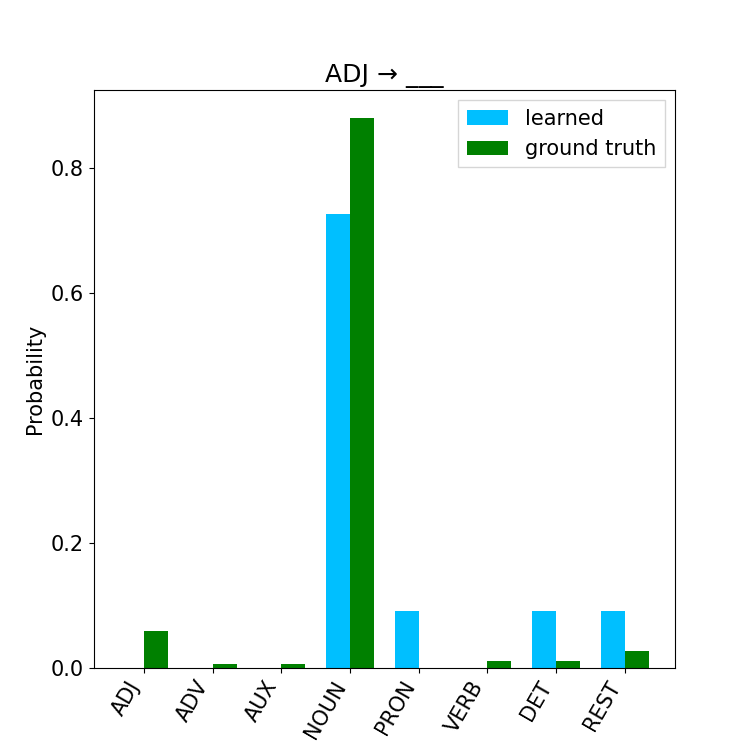
\includegraphics[width=\twocolpicwidth]{Bilder/chapter4/Barplots/Avg_OHE_OHE_5000E_100BS_1L_1C_200P_1500T_D/_epoch-4000//Combined_Barplot_ADJ_F.png}
		}
	\caption{Comparison of the averaged predictions (green) with the ground truth distribution (blue). The model was trained by \onehot{s} and german data. If a \postag{} has no blue bar, it has a $ 0 $\% probability to appear as successor \eg after an \texttt{ADJ} comes no \texttt{ADP}. The remaining plots of the other \postag{s} can be found in \appref{ch: appendix average approach}.}
	\label{fig: barplot det adp}
\end{figure}
\begin{table}
	\centering
	\caption[Schematic sentences for \postag{} rules]{Schematic sentences of the book used in \figref{\ref{fig: barplot det adp}}.}
	\begin{tabular}{l|l}
		\toprule
		Rule				& Sentence \\
		\midrule
		\texttt{ADP → NOUN}	& Sie hat mich \texttt{zum Schmunzeln}
		gebracht. \\
		\texttt{ADP → PRON}	& Es war überaus angenehm,
		sich \texttt{mit Ihnen} zu unterhalten. \\
		\texttt{ADP → DET}	& Ich bin nämlich eine gebürtige Linkshänderin,
		die \texttt{in der} Schule, [...] \\
		%%
		%		\texttt{DET → NOUN}	& \texttt{Das Werkzeug}, das im Keller liegt, [...] \\
		%		\texttt{DET → ADV}	& \texttt{Ein gut} ausgestattetes Museum, [...] \\
		%		\texttt{DET → ADP}	& Das Werkzeug, \texttt{das im} Keller liegt, [...] \\
		%
		\texttt{ADJ → NOUN}	& Lieber Leo, ich habe drei \texttt{fürchterliche Tage} hinter mir. \\
		\bottomrule
	\end{tabular}
	\label{tab: example sentences}
\end{table}

% --------------------------------------

\subsection{Averaging models: Evaluating the results}
The same configurations as in \secreff{subsec: text model evaluating the results} were processed. By ``configurations'' is subsumed: german and english, \onehot{} or word vector version and the same number of epochs and words used for training. After the unsatisfactory performance of the word vector approaches (\tabref{\ref{tab: text model versions and metrics}}), everything else than a similar outcome would be surprising. A detailed illustration of the results offers \figref{\ref{fig: rsme plots}}. By this plot it is also possible to talk about the outcomes a bit more specifically.
%
\begin{figure}
	\centering
		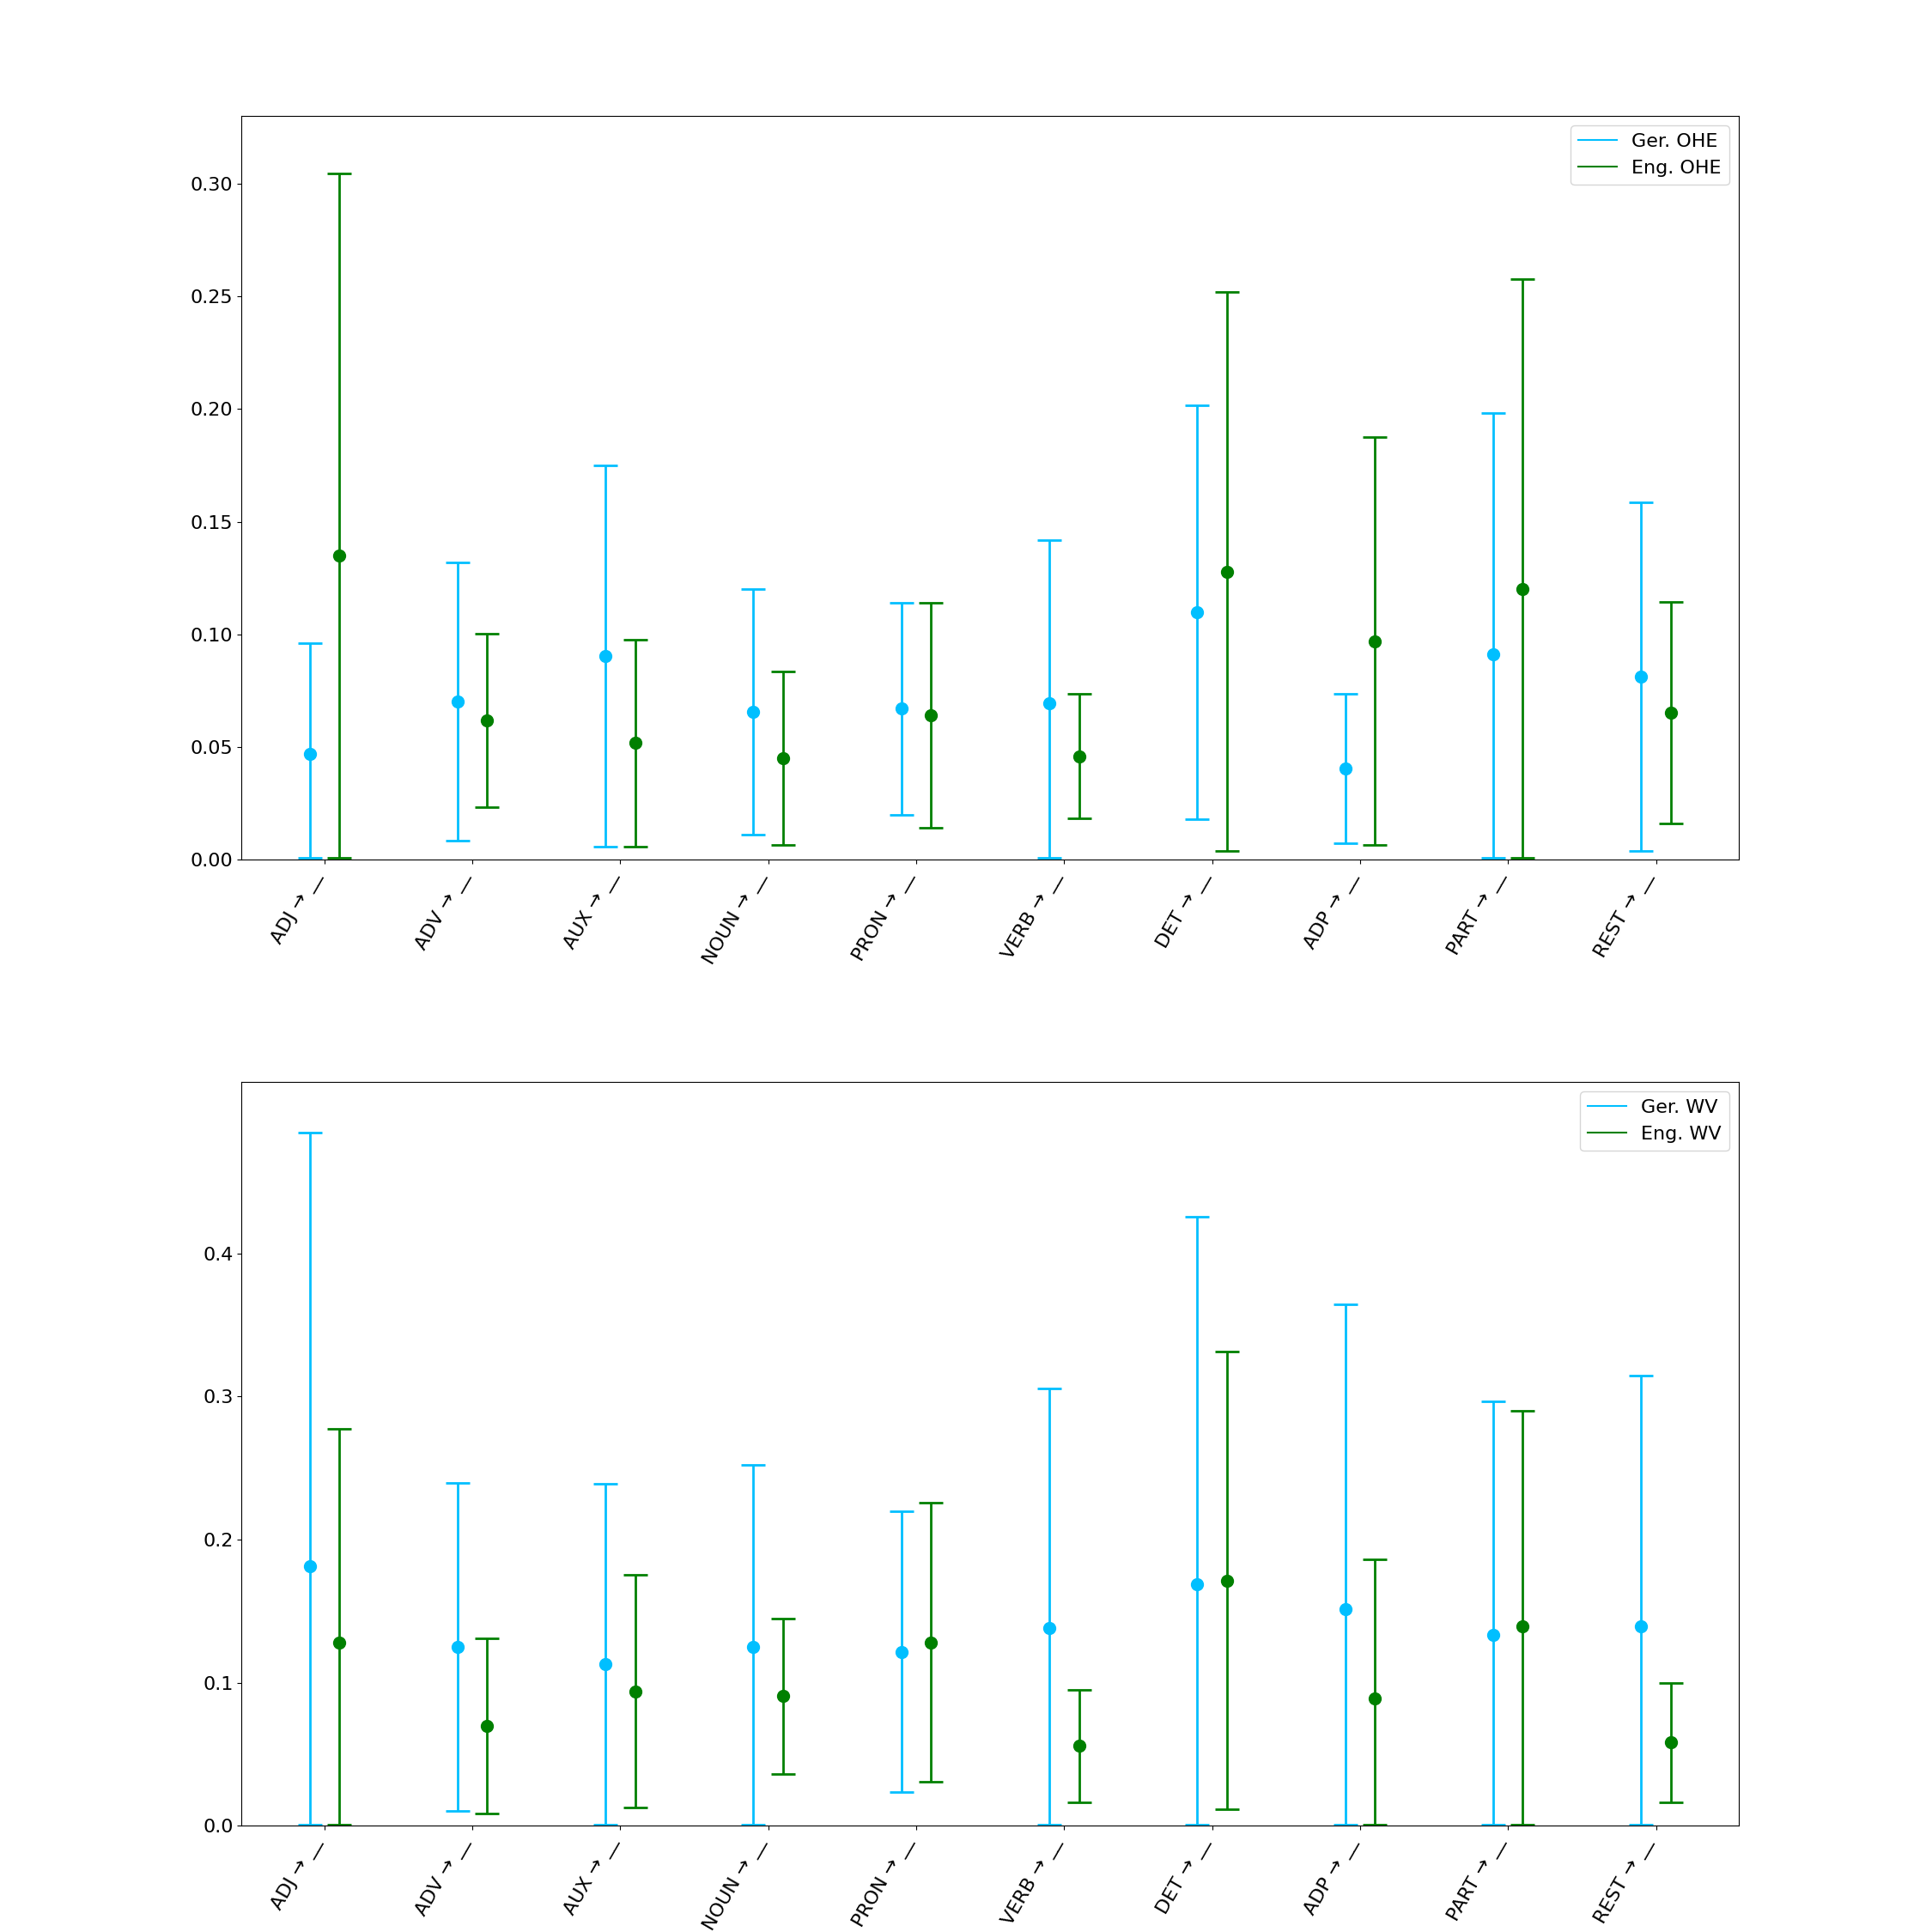
\includegraphics[scale=0.325, center]{code/error_com.png}
	\caption{Mean and standard deviation of the configurations \wrt to the ground truth \ie the difference between the ground truth matrix and the prediction matrix was used for the row wise calculations (matrices depicted in \figref{\ref{fig: avg model gt w2v de en}}). Clearly visible that \onehot{} models (OHE) outperform word vector versions (WV). Both, mean and standard deviation, are lower. Because a difference is assessed, smaller means are better.}
	\label{fig: rsme plots}
\end{figure}
All means are to some extent equal but the standard deviations differ. The free word order of German doesn't seem to be a problem because both models learn better than their English counterparts (\tabref{\ref{tab: avg model versions and metrics}}). There are some difficulties with adjectives (except for Ger. OHE), although they are tied to \texttt{NOUN} and \texttt{ADJ} (\figref{\ref{fig: barplot det adp}}).

Sadly, the prepared visualizations \ie \figref{\ref{fig: rsme plots}} and \tabref{\ref{tab: avg model versions and metrics}}, lack the ability to grasp the full picture: The word vector configurations seem to work by checking the means for each \postag{}, but when inspecting the matrices as a whole as in \figref{\ref{fig: avg model gt w2v de en}}, it is apparent that they don't. Whereas using the english book, the model degenerates to the identical distribution and the german one contemplates \texttt{NOUN} as its personal $ 42 $.
%By checking the averaged means of \figref{\ref{fig: rsme plots}} in \tabref{\ref{tab: avg model versions and metrics}}, it is unexpected that the english word vector model has a far lower value and is closer to \onehot{} variant than to the german equivalent. An impression which can also gained by \figref{\ref{fig: rsme plots}}. Although not comparable by mere numbers but rather qualitatively the score should be located closer to the other word vector model as in \tabref{\ref{tab: text model versions and metrics}} because the model structure is the same. This anomaly can be explained by inspecting the transition matrix as a whole as in \figref{\ref{fig: transitionprobabilitymatrixt1df0}}. It more or less resembles an identical distribution.
%
%Therefore, the low value of the english \onehot{} model is explained by the identically distributed predictions in this row.
\begin{table}
	\centering
	\caption{Averaged means of the difference between prediction and ground truth. As expected, the word vector versions have higher scores than the \onehot{} counterpart. These values can't be used for a comparison with \tabref{\ref{tab: text model versions and metrics}} because the underlying metrics are different.}
	\begin{tabular}{lll}
		\toprule
		Version					& Mean in $ 10^{-2} $	& Standard deviation in $ 10^{-2} $ \\
		\midrule
		german, \onehot{} 		& $ 7.3 $				& $ 2.0 $ \\% 0.08200
		german, word vector		& $ 14.0 $				& $ 2.1 $ \\% 0.74139
		english, \onehot{}		& $ 8.1 $				& $ 3.3 $ \\% 0.10021
		english, word vector	& $ 10.2 $				& $ 3.6 $ \\% 0.77522
		\bottomrule
	\end{tabular}
	\label{tab: avg model versions and metrics}
\end{table}
%
%As expected, the word vector versions have higher scores than the \onehot{} counterpart. Again, the german training data reached the best value, which makes sense after checking \figref{\ref{fig: avg model ohe de en tpm} and \ref{fig: avg model w2v de en tpm}}. Due to the more flexible sentence structure this was unforeseeable. Although derived from the illustration the approaches using word vectors don't seem to learn anything. Despite being close to its \onehot{} counterpart, the english word vector version seem to approach an identical distribution, whereas training with german word vectors (\figref{\ref{fig: avg model w2v de en tpm}}) fails completely and concentrates on \texttt{NOUN} as its personal $ 42 $.
%
\begin{figure}
	\centering
		\subcaptionbox{German, ground truth of word class transitions.}{
			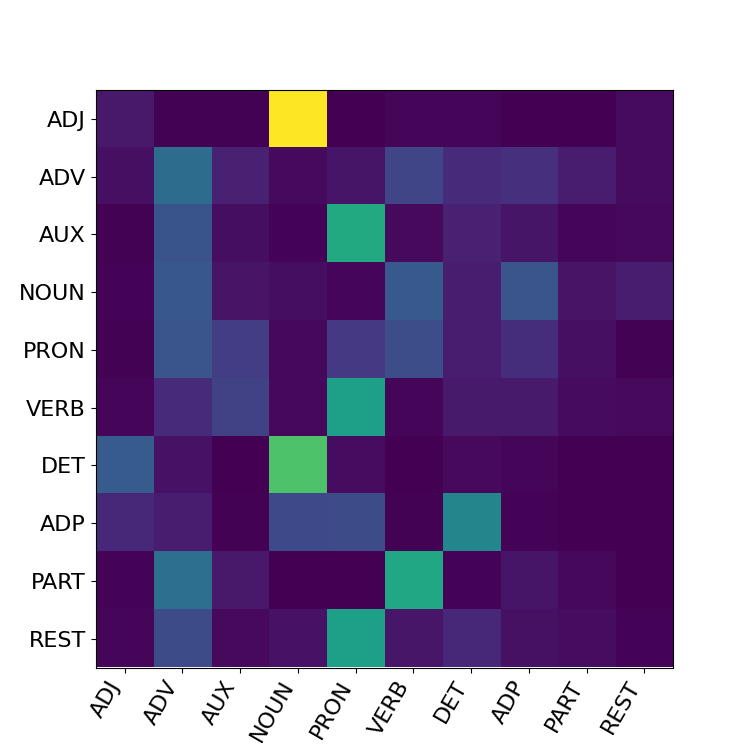
\includegraphics[height=\threerowpicheight]{Bilder/chapter4/average_models/ground_truths/D_200pages_1500T_tags.png}
		}
		\hspace*{1cm}
		\subcaptionbox{English, ground truth of word class transitions.}{
			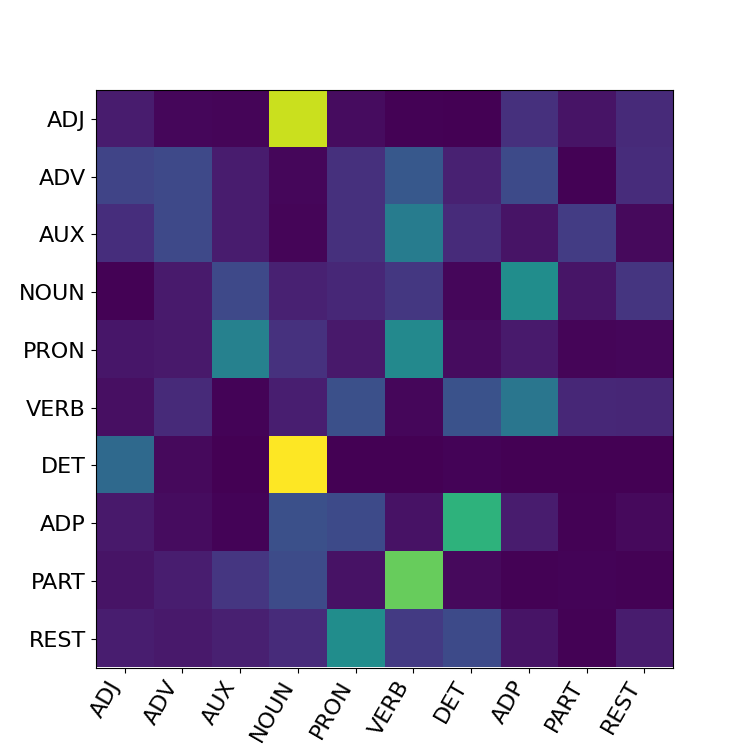
\includegraphics[height=\threerowpicheight]{Bilder/chapter4/average_models/ground_truths/J_200pages_1500T_tags.png}
		}
		\\
		\subcaptionbox{German, learned \gls{sr} using \onehot{s}.}{
			\includegraphics[height=\threerowpicheight]{Bilder/chapter4/average_models/plots/Avg_OHE_OHE_5000E_100BS_1L_1C_200P_1500T_D/_epochs-4000/Transition_Probability_Matrix;_t=1,_DF=0.5.png}
		}
		\hspace*{1cm}
		\subcaptionbox{English, learned \gls{sr} using \onehot{s}.}{
			\includegraphics[height=\threerowpicheight]{Bilder/chapter4/average_models/plots/Avg_OHE_OHE_4000E_100BS_1L_1C_200P_1500T_J/Transition_Probability_Matrix;_t=1,_DF=0.5.png}
		}
		\\
		\subcaptionbox{German, learned \gls{sr} using word vectors.}{
			\includegraphics[height=\threerowpicheight]{Bilder/chapter4/average_models/plots/Avg_W2V_W2V_5000E_100BS_1L_1C_200P_1500T_D/_epochs-4000/Transition_Probability_Matrix;_t=1,_DF=0.5.png}
		}
		\hspace*{1cm}
		\subcaptionbox{English, learned \gls{sr} using word vectors.}{
			\includegraphics[height=\threerowpicheight]{Bilder/chapter4/average_models/plots/Avg_W2V_W2V_5000E_100BS_1L_1C_200P_1500T_J/_epochs-4000/Transition_Probability_Matrix;_t=1,_DF=0.5.png}
		}
	\caption{If word vectors are used for training the model has problems with both languages. When using German the predictions degenerate completely and will classify everything as \texttt{NOUN}. The outcome of precessing English is reversed: it is quite close to an identical distribution which equals mere guessing amidst the \postag{s}.}
	\label{fig: avg model gt w2v de en}
\end{figure}

%\begin{table}[H]
%	\centering
%	\caption{For each row of the learned matrices the \gls{rmse} was calculated according to the corresponding ground truth. The values mustn't be compared to \tabref{\ref{tab: text model versions and metrics}} since they were calculated differently. Last row show the average over the columns. Meaning of the acronyms: OHE = \onehot{}, WV = word vector.}
%	\begin{tabular}{lcccc}
%		\toprule
%		Transition & Ger. OHE & Ger. WV & Eng. OHE & Eng. WV \\
%		\midrule
%		\texttt{ADJ → \_\_\_}	& 0.15 & 0.79 & 0.48 & 0.44 \\
%		\texttt{ADV → \_\_\_}	& 0.20 & 0.38 & 0.16 & 0.21 \\
%		\texttt{AUX → \_\_\_}	& 0.27 & 0.38 & 0.15 & 0.28 \\
%		\texttt{NOUN → \_\_\_}	& 0.19 & 0.40 & 0.13 & 0.24 \\
%		\texttt{PRON → \_\_\_}	& 0.18 & 0.35 & 0.18 & 0.36 \\
%		\texttt{VERB → \_\_\_}	& 0.22 & 0.49 & 0.12 & 0.15 \\
%		\texttt{DET → \_\_\_}	& 0.32 & 0.69 & 0.40 & 0.52 \\
%		\texttt{ADP → \_\_\_}	& 0.12 & 0.58 & 0.30 & 0.29 \\
%		\texttt{PART → \_\_\_}	& 0.31 & 0.47 & 0.41 & 0.46 \\
%		\texttt{REST → \_\_\_}	& 0.25 & 0.50 & 0.19 & 0.16 \\
%		\hline
%		$ \varnothing $ & 0.21 & 0.50 & 0.25 & 0.31 \\
%		\bottomrule
%	\end{tabular}
%	\label{tab: avg model versions and metrics}
%\end{table}


% === CONCLUSION ===================================

\section{Conclusion}
\begin{frame}{Conclusion}
    \begin{itemize}
        \item<+-> By far most of the time was consumed by finding proper values, sadly with bad luck
        \item<+-> Plenty of configurations didn't improve the results or were worse. Two of them were
        \begin{itemize}
            \item<+-> Multiple hidden layers
            \item<+-> Predicting only most frequent words
        \end{itemize}
        \item<+-> Due to the lack of valid data from real experiments interpretation regarding our daily life is difficult
        \item<+-> Performance of word vectors disappointing, which is a drawback because they might be closer to actual signals
        \item<+-> Some learning does happen (Average approach)
    \end{itemize}
    \begin{figure}
        \centering
            \includegraphics<7->[height=0.4\textheight]{Bilder/average_models/ground_truths/D_200pages_1500T_tags.png}
            \includegraphics<7->[height=0.4\textheight]{Bilder/average_models/Avg_OHE_OHE_5000E_100BS_1L_1C_200P_1500T_D/Transition_Probability_Matrix;_t=1,_DF=0.5.png}
    \end{figure}

% --- NOTIZEN -----------------------------------
\mynote{
    \begin{itemize}
        \item[ü] Coming to the Conclusion
        \item By far most of the time was consumed by finding well functioning values.
        \item Plenty of configurations didn't improve the results or were worse. Although it took much space during the months the dead ends aren't illustrated in the presentation but in the thesis. Two of them were
        \begin{itemize}
            \item Multiple hidden layers
            \item Predicting only most frequent words
        \end{itemize}
        \item Due to the lack of valid data from real experiments interpretation regarding our daily life is difficult
        \item Unfortunately, performance of word vectors is in general disappointing, which is a drawback because they might be closer to actual signals
        \item Nevertheless, some learning does happen and paths can be reconstructed (Average approach) ENDE DES VORTRAGS
    \end{itemize}
}
\end{frame}

% === REFERENCES ===================================

\section*{References}
\begin{frame}[allowframebreaks,noframenumbering]{References}
	\printbibliography
\end{frame}
%}

\finalframe{Thank you\\for your attention!}

\end{document}
